%% Version 5.0, 2 January 2020
%
%%%%%%%%%%%%%%%%%%%%%%%%%%%%%%%%%%%%%%%%%%%%%%%%%%%%%%%%%%%%%%%%%%%%%%
% TemplateV5.tex --  LaTeX-based template for submissions to the 
% American Meteorological Society
%
%%%%%%%%%%%%%%%%%%%%%%%%%%%%%%%%%%%%%%%%%%%%%%%%%%%%%%%%%%%%%%%%%%%%%
% PREAMBLE
%%%%%%%%%%%%%%%%%%%%%%%%%%%%%%%%%%%%%%%%%%%%%%%%%%%%%%%%%%%%%%%%%%%%%

%% Start with one of the following:
% DOUBLE-SPACED VERSION FOR SUBMISSION TO THE AMS
\documentclass{ametsocV5}

% TWO-COLUMN JOURNAL PAGE LAYOUT---FOR AUTHOR USE ONLY
% \documentclass[twocol]{ametsocV5}


% Enter packages here. If too many math alphabets are used,
% remove unnecessary packages or define hmmax and bmmax as necessary.

%\newcommand{\hmmax}{0}
%\newcommand{\bmmax}{0}
\usepackage{amsmath,amsfonts,amssymb,bm}
\usepackage{mathptmx}%{times}
\usepackage{newtxtext}
\usepackage{newtxmath}


%%%%%%%%%%%%%%%%%%%%%%%%%%%%%%%%

%%% To be entered by author:

%% May use \\ to break lines in title:

\title{Southern Ocean heat storage, reemergence and winter sea-ice decline induced by summertime winds.}

%%% Enter authors' names, as you see in this example:
%%% Use \correspondingauthor{} and \thanks{Current Affiliation:...}
%%% immediately following the appropriate author.
%%%
%%% Note that the \correspondingauthor{} command is NECESSARY.
%%% The \thanks{} commands are OPTIONAL.

    %\authors{Author One\correspondingauthor{Author name, email address}
% and Author Two\thanks{Current affiliation: American Meteorological Society, 
    % Boston, Massachusetts.}}

\authors{Edward W. Doddridge\correspondingauthor{Edward W. Doddridge, edward.doddridge@utas.edu.au}}

%% Follow this form:
    % \affiliation{American Meteorological Society, 
    % Boston, Massachusetts}

\affiliation{Earth, Atmospheric and Planetary Sciences,
Massachusetts Institute of Technology,
77 Massachusetts Avenue,
Cambridge, 02139,
USA, and Institute for Marine and Antarctic Studies, University of Tasmania,
20 Castray Esplanade,
Hobart, 7001,
Australia}

\extraauthor{John Marshall}
\extraaffil{Earth, Atmospheric and Planetary Sciences,
Massachusetts Institute of Technology,
77 Massachusetts Avenue,
Cambridge, 02139,
USA}

\extraauthor{Hajoon Song}
\extraaffil{Department of Atmospheric Sciences,
Yonsei University,
50 Yonsei-ro, Seodaemun-gu,
Seoul, 03722, South Korea}

\extraauthor{Jean-Michel Campin}
\extraaffil{Earth, Atmospheric and Planetary Sciences,
Massachusetts Institute of Technology,
77 Massachusetts Avenue,
Cambridge, 02139,
USA}

\extraauthor{Maxwell Kelley}
\extraaffil{NASA Goddard Institute for Space Studies,
2880 Broadway,
New York, NY 10025 USA}
%% If appropriate, add additional authors, different affiliations:
    %\extraauthor{Extra Author}
    %\extraaffil{Affiliation, City, State/Province, Country}

%\extraauthor{}
%\extraaffil{}

%% May repeat for a additional authors/affiliations:

%\extraauthor{}
%\extraaffil{}

%%%%%%%%%%%%%%%%%%%%%%%%%%%%%%%%%%%%%%%%%%%%%%%%%%%%%%%%%%%%%%%%%%%%%
% ABSTRACT
%
% Enter your abstract here
% Abstracts should not exceed 250 words in length!
%
 

\abstract{The observational record shows a substantial 40-year upward trend in summertime westerly winds over the Southern Ocean, as characterised by the Southern Annular Mode (SAM) index. Enhanced summertime westerly winds have been linked to cold summertime sea surface temperature (SST) anomalies. Previous studies have suggested that an Ekman transport mechanism is responsible for this seasonal cooling. Here, another equally important process is presented in which cooling, driven by summertime wind-induced enhanced vertical mixing, moves heat downwards, cooling the sea surface and warming subsurface waters. The anomalously cold SSTs draw heat from the atmosphere into the ocean, leading to enhanced depth-integrated ocean heat content. The subsurface heat is returned to the surface mixed layer during the autumn and winter as the mixed layer deepens, leading to anomalously warm SSTs and potentially reducing sea ice cover. Observational analyses and numerical experiments support this mechanism, showing that enhanced vertical mixing drives subsurface warming and cools the surface mixed layer. Anomalous advection also contributes to the surface cooling, but the relative importance of advective and mixing contributions is model dependent. Modeling results suggest that sea ice volume is more sensitive to summertime winds than sea ice extent, implying that enhanced summertime westerly winds may lead to thinner sea ice in the following winter, if not lesser ice extent. Thus, strong summertime winds could precondition the sea ice cover for a rapid retreat in the following melt season.
}

\begin{document}

%% Necessary!
\maketitle

%%%%%%%%%%%%%%%%%%%%%%%%%%%%%%%%%%%%%%%%%%%%%%%%%%%%%%%%%%%%%%%%%%%%%
% SIGNIFICANCE STATEMENT/CAPSULE SUMMARY
%%%%%%%%%%%%%%%%%%%%%%%%%%%%%%%%%%%%%%%%%%%%%%%%%%%%%%%%%%%%%%%%%%%%%
%
% If you are including an optional significance statement for a journal article or a required capsule summary for BAMS 
% (see www.ametsoc.org/ams/index.cfm/publications/authors/journal-and-bams-authors/formatting-and-manuscript-components for details), 
% please apply the necessary command as shown below:
%
% \statement
% Significance statement here.
%
% \capsule
% Capsule summary here.


%%%%%%%%%%%%%%%%%%%%%%%%%%%%%%%%%%%%%%%%%%%%%%%%%%%%%%%%%%%%%%%%%%%%%
% MAIN BODY OF PAPER
%%%%%%%%%%%%%%%%%%%%%%%%%%%%%%%%%%%%%%%%%%%%%%%%%%%%%%%%%%%%%%%%%%%%%
%


\section{Introduction}


% Things to add to the paper:
% \begin{itemize}
%     \item Relevance to polynya formation \citep{Wilson2019,Kurtakoti2018} - enhanced mixing increases salinity of the mixed layer (during summer). Is that relevant? Need to look at evolution of mixed layer depth over the seasonal cycle. Salinity anomalies seem to be important when advected in horizontally \citep{Kurtakoti2018}, but less clear if they are important when generated by anomalous vertical mixing
%     \item Stratification from freshwater fluxes (and possible compensation between wind-driven mixing that deepens the mixed layer and freshwater fluxes that shoal the mixed layer) \citep{Wilson2019}.
%     \item SAM influences on clouds and precip
%     \item Sea ice changes and associated freshwater fluxes \citep{Haumann2016}.
%     \item Emphasize this is about summertime winds. What would wintertime winds do?
% \end{itemize}

Each year approximately 15 million square kilometers of sea ice forms and subsequently melts in the seasonal ice zone of the Southern Ocean \citep{Fetterer2016}. The buoyancy fluxes associated with this seasonal ice cycle play an important role in the meridional overturning circulation in the Southern Ocean \citep{Abernathey2016,Haumann2016}. This connects the surface with the abyss and is a conduit for exchange between reservoirs of heat, carbon, and nutrients \citep{Sarmiento2004} in the ocean and the atmosphere. To predict how the climate system will respond to anthropogenic influences we need to be able to capture changes to the overturning circulation which itself demands understanding of the processes that affect the seasonal growth and decay of sea ice in the Southern Ocean.

Sea ice extent around Antarctica has exhibited a gradual increase from the beginning of the satellite record in the late 1970s. This is likely to be causally linked to the strengthening of the surface westerlies blowing around Antarctica during the same period. As described by, for example, \citet{Ferreira2015}, \citet{Purich2016}, \citet{Doddridge2017} and \citet{Kostov2017}, the enhanced summertime westerly winds associated with the positive phase of the SAM lead to a rapid cooling of the SST on a timescale of weeks to months. Two advective mechanisms have been proposed to explain the cold summertime SST anomalies associated with a positive summertime SAM: anomalous northwards Ekman transport moving fluid across the meridional temperature gradient \citep{Ferreira2015,Kostov2017}, and anomalous vertical advection due to Ekman pumping drawing cold subsurface water upwards into the mixed layer \citep{Purich2016}. In contrast to these two advective mechanisms, \citet{Doddridge2019a} suggested that enhanced near surface vertical mixing may contribute to the cold surface anomalies by mixing surface heat to depth, creating anomalously warm temperatures just below the zonal-mean mixed layer depth. In an observational study, \citet{Doddridge2017} showed that cold summertime SST anomalies associated with a positive summertime SAM lead to enhanced growth of sea ice in the autumn. The data suggested that there may also be a small reduction in sea ice extent at the wintertime maximum. However, substantial interannual variability and a relatively short observational record, prevented the identification of a statistically significant signal in wintertime sea ice extent. Motivated by the observational analysis of \citet{Doddridge2017} and the enhanced mixing reported by \citet{Doddridge2019a}, we return to these themes in this paper. 

As summarised in Figure \ref{fig:wind_mixing_schematic}, we propose a vertical-mixing mechanism in which summertime wind anomalies sequester heat below the mixed layer, cooling the surface. This draws heat in to the surface ocean from the atmosphere adding to the heat stored in the column. As the mixed layer deepens in the autumn and winter, this heat sequestered in the summer reemerges, warming SSTs, reducing sea-ice volume and potentially sea ice cover. We explore these ideas in the observations, in an idealised channel model of the seasonal ice zone, and in a comprehensive coupled climate model.


\begin{figure}[!ht]
    \begin{center}
        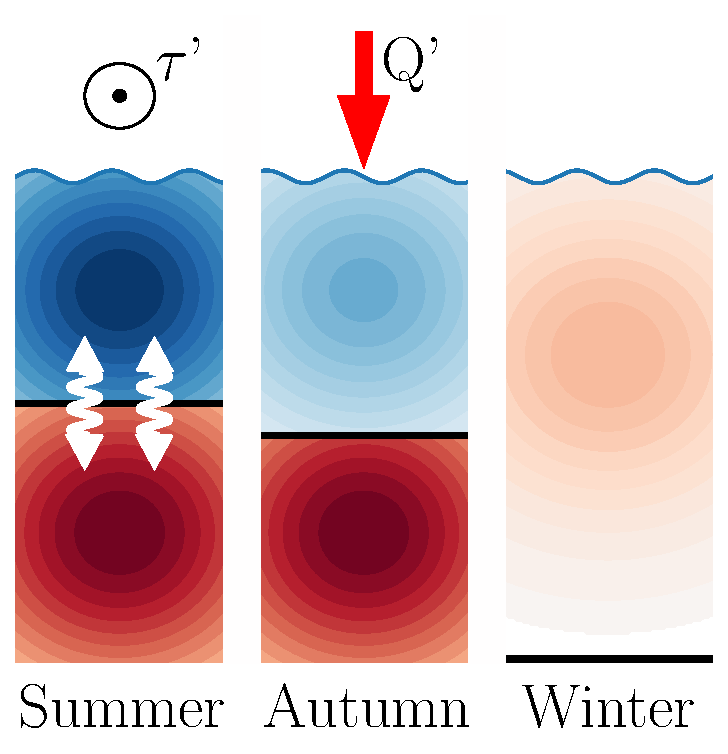
\includegraphics[width=0.7\textwidth]{figures/wind_mixing_schematic.pdf}
        \caption{Schematic of vertical mixing/heat sequestration mechanism. In summer, anomalous westerly winds ($\tau^{'}$ above left hand column) enhance vertical mixing at the base of the mixed layer (white squiggly arrows and horizontal black line, respectively) moving heat downwards and causing a vertical dipole of anomalous temperatures (colors). The anomalously cold SST causes anomalous heat fluxes into the ocean during the autumn ($Q^{'}$ and red arrow above central column), which reduces the cold SST anomaly. As autumn progresses, the mixed layer continues to deepen, entraining the anomalously warm fluid sequestered below the zonal-mean mixed layer depth. Due to the anomalous surface heat fluxes, which increases the total heat content of the upper ocean, the mixed layer is now anomalously warm. This can be expected to lead to a reduction in wintertime sea ice.}
        \label{fig:wind_mixing_schematic}
    \end{center}
\end{figure}


Our paper is set out as follows. In section \ref{sec:subsurface_heat_sequestration} we describe the climatology of the Southern Ocean and present our new mechanism. In section \ref{sec:analysis_of_observations} we analyse observational datasets and find some evidence to support our new mechanism. In an effort to reduce the uncertainties in our analysis we turn to numerical models in sections \ref{sec:analysis_of_an_idealised_channel_model} and \ref{sec:analysis_of_a_global_coupled_model}, where we find strong evidence that enhanced summertime winds lead to increased vertical mixing and the subsurface sequestration of heat. We then summarise our findings and present our conclusions in section \ref{sec:discussion}.





% % , moving heat downwards into the subsurface ocean.

% There is a long history of exploring the dynamics of the Southern Ocean with zonal-mean theories \citep[e.g.][]{Marshall2003}, and while the idea that regional variations are too important to neglect has been gaining traction \citep[see e.g.][]{Rintoul2018,Tamsitt2017,Thompson2012,Viebahn2012,Viglione2016}, there are still contributions to be made by considering the zonal-mean dynamics of the Southern Ocean. Understanding the zonal-mean response is especially relevant when considering the response of the ocean and sea ice to hemisphere scale forcings such as the Southern Annular Mode (SAM). The SAM is the dominant mode of variability in the extratropical southern hemisphere \citep{Gong1999,Thompson2000} and the positive phase of the SAM is associated with a strengthening and poleward shift of the midlatitude westerly winds \citep{Thompson2000}.

% \citet{Ferreira2015} suggested that the surface cooling was caused by anomalous northward Ekman transports, while \citet{Purich2016} suggested that strengthened westerly winds would lead to enhanced upwelling of winter water into the mixed layer, thereby cooling the surface of the ocean. \citet{Doddridge2017} used observations to explore the surface response of the Southern Ocean to summertime SAM anomalies. They investigated changes to the zonal-mean SST and sea ice extent in the Southern Ocean. \citet{Doddridge2017} showed that a positive summertime SAM was followed by cold SST anomalies and a transient increase in sea ice extent during the fall. Their results hint at a possible reduction in sea ice extent from July onwards, but the large uncertainties preclude the possibility of significant results (see their figure 3). \citet{Doddridge2019a} used Argo observations and numerical models to explore the subsurface response of the Southern Ocean to westerly wind perturbations. In addition to the expected SST cooling, they found a subsurface warming and attributed it to enhanced vertical mixing at the base of the mixed layer.

% \citet{Doddridge2019a} showed that the subsurface warming was due to enhanced vertical mixing caused by the wind perturbation. In the summertime, the surface of the Southern Ocean is characterized by a thin mixed layer of warmer water overlying the cold remnants of the previous winter's mixed layer. As such, any enhanced vertical mixing at the base of the mixed layer will act to cool the mixed layer and warm the fluid below, moving heat downwards in the water column. In addition to the zonal-mean heat budget analysis presented by \citet{Doddridge2019a}, we can use the integrated heat content anomalies to infer the mechanism responsible for the cooling in the mixed layer and the warming below it. If the heat content deficit in the mixed layer is the same magnitude as the anomalous heat content below the zonal-mean mixed layer depth, then it is highly likely that enhanced vertical mixing, rather than anomalous horizontal or vertical advection, has caused the temperature anomalies.





% section introduction (end)


\section{Vertical mixing and the seasonal sequestration of heat} % (fold)
\label{sec:subsurface_heat_sequestration}

The time-mean circulation of the extratropical atmosphere in the southern hemisphere is dominated by a strong westerly jet over the Southern Ocean (figure \ref{fig:zonal_wind_clim}). Surface winds are the major source of energy for the oceanic circulation \citep{Wunsch1998} and contribute substantially to mixing \citep{Munk1998}, including to the formation of the surface mixed layer \citep{Pollard1972,Wunsch2004}. The variability of the atmospheric circulation in the southern hemisphere is dominated by the Southern Annular Mode (SAM) \citep{Gong1999,Thompson2000}. The positive phase of the SAM is associated with a strengthening and poleward shift of the midlatitude westerly winds \citep{Thompson2000}. Both the summertime and annual mean SAM have become increasingly positive since the middle of the 20th Century \citep{Jones2016,Marshall2003a} due to anthropogenic emissions of ozone depleting substances and greenhouse gases \citep[see e.g.][]{Polvani2011,Swart2012,Thompson2011a}.


\begin{figure}[!ht]
    \begin{center}
        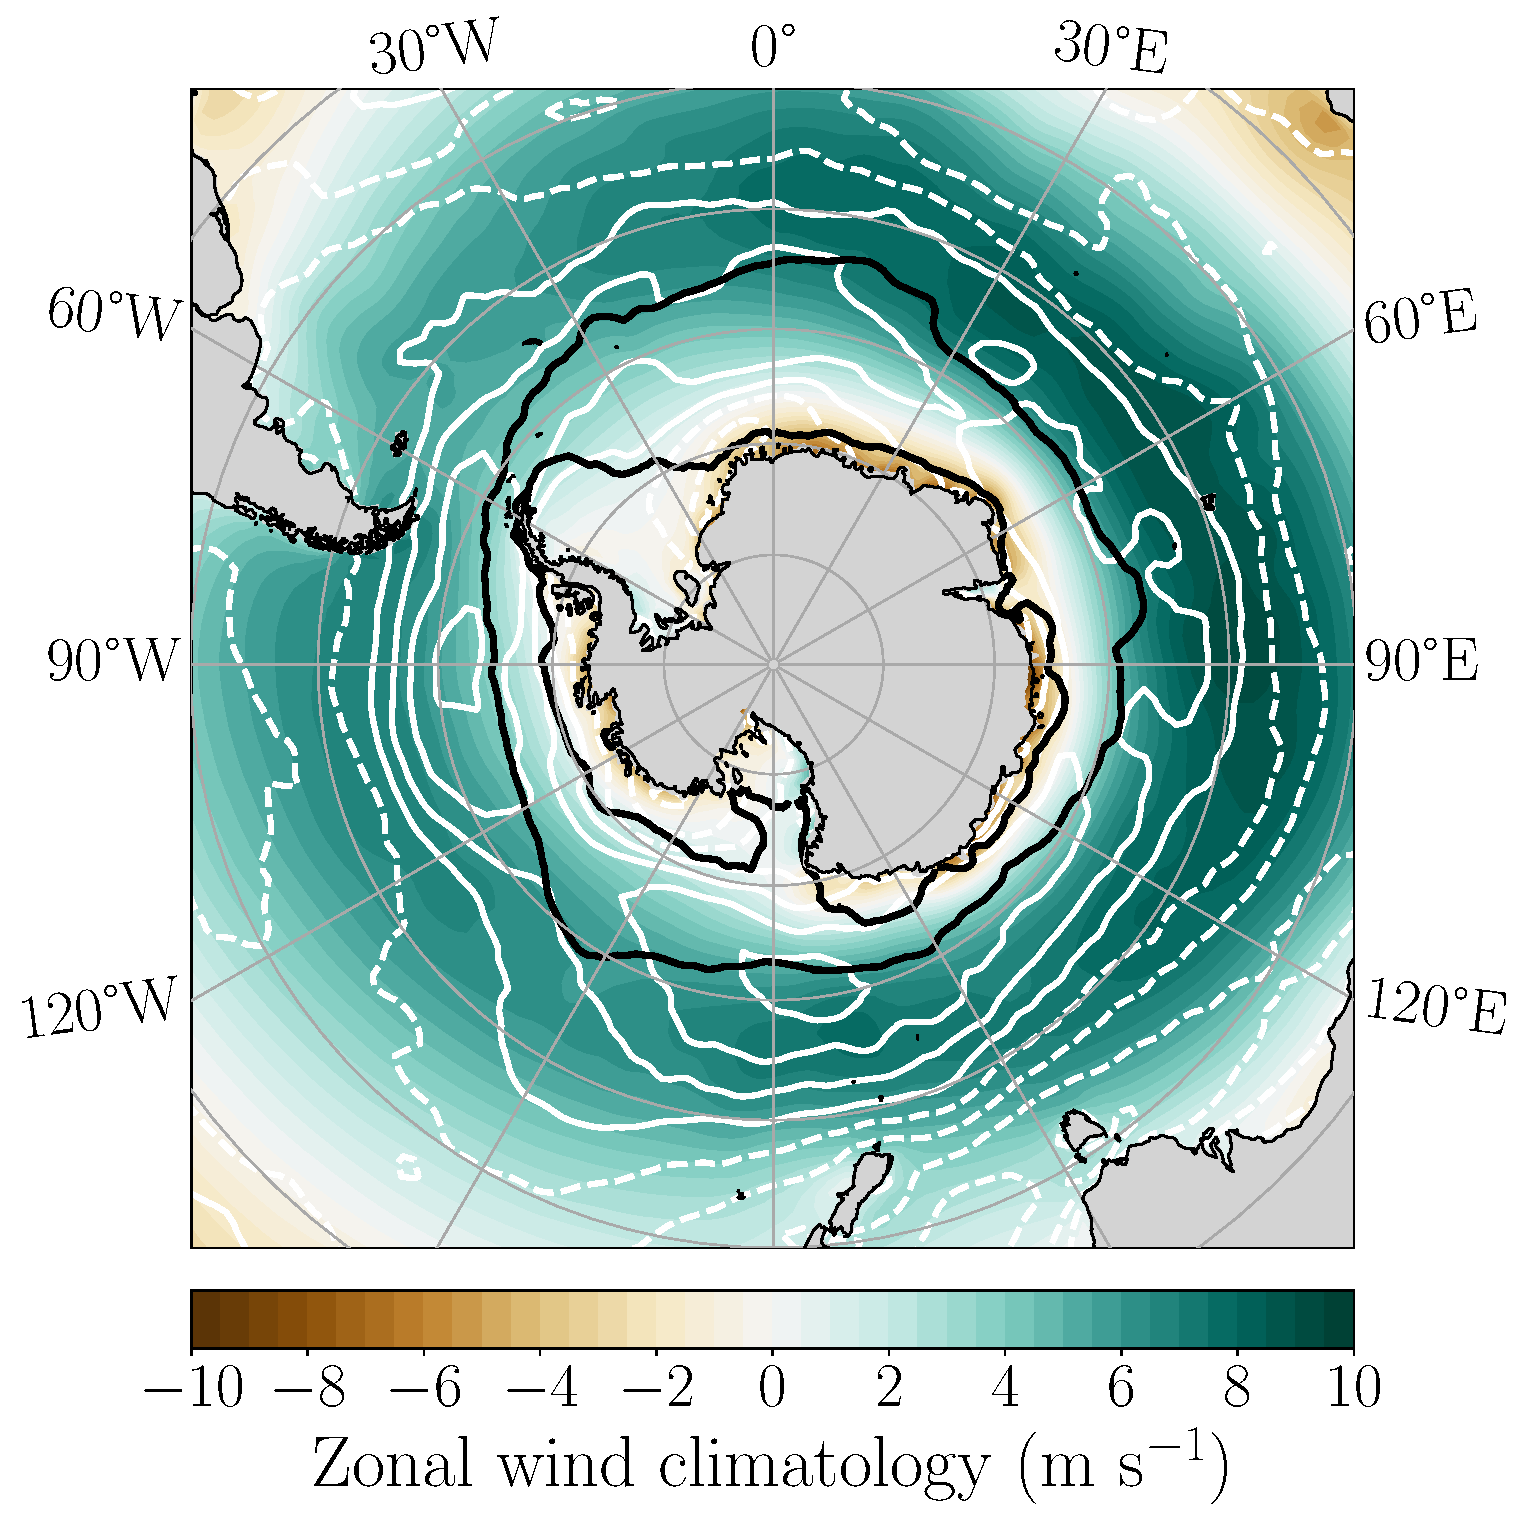
\includegraphics[width=0.7\textwidth]{figures/zonal_wind_clim.pdf}
        \caption{Climatology of the Southern Ocean. Annual mean zonal wind (colors), wind anomaly associated with a +1 summertime Southern Annular Mode (SAM) anomaly (white contours, contour interval is 0.2 m s$^{-1}$, negative contours dashed), and seasonal sea ice edges for the summer minimum and winter maximum (defined as the 15\% concentration contour, black contours).}
        \label{fig:zonal_wind_clim}
    \end{center}
\end{figure}

The positive trend in the SAM over the latter part of the 20th century \citep{Jones2016} has contributed to an increase in wind stress variance and more near inertial energy in the Southern Ocean \citep{Rath2014}. This near inertial wind stress variability has a large impact on the circulation of the Southern Ocean \citep{Munday2017} and generates near-inertial waves that increase mixing in the upper ocean \citep{Furuichi2008,Rath2014,Song2019,Zhai2009}. We should therefore expect that the zonal wind changes associated with the SAM will affect the depth of the surface mixed layer. This intuition is supported by the results of \citet{Panassa2018}, who found that the stronger zonal winds associated with the positive phase of the SAM leads to deeper summertime mixed layers in the Southern Ocean.

The Southern Ocean mixed layer serves as a gateway between the subsurface ocean and the atmosphere \citep{Klocker2018,Marshall1997a} and the seasonal cycle in the depth of the mixed layer regulates a range of physical and biogeochemical processes \citep{Doney2004,Williams2017}. The Southern Ocean mixed layer is shallowest during the summer months \citep{Holte2017}, when the cold remnants of the previous winter's mixed layer are capped by a warmer surface layer. This thermal structure is crucial for our mechanism, since it supplies a large reservoir of cold water that can be readily accessed by the surface mixed layer. Any process that acts to deepen the summertime mixed layer will cool the surface waters and warm the fluid that was previously below the base of the summertime mixed layer.

\citet{Doddridge2019a} found that stronger westerly winds associated with the positive phase of the SAM created a region of warming just below the zonal-mean mixed layer depth in both observations and models. A heat budget analysis of their simulations showed that this warming was due to enhanced vertical mixing. Since mixing can only redistribute heat, this enhanced vertical mixing must also contribute to the observed surface cooling that has previously been ascribed to purely advective mechanisms \citep{Ferreira2015,Purich2016}. The presence of anomalously cold water at the sea surface will affect air-sea heat fluxes; if the surface ocean is anomalously cold, then the air-sea heat flux feedback will act to reduce the SST anomaly by transferring heat from the atmosphere into the ocean \citep{Hausmann2017a}. We therefore expect an anomalously cold surface ocean to absorb additional heat from the atmosphere, leading to a positive depth integrated ocean heat content anomaly. As the mixed layer deepens during autumn and winter, the subsurface heat will be returned to the surface where it may affect the growth of sea ice and reduce sea ice extent or volume. Our proposed mechanism is summarized schematically in figure \ref{fig:wind_mixing_schematic}. In the following sections we use observational datasets and numerical experiments to test our proposed mechanism and explore the relationship between the SAM, zonal-mean temperature, and sea ice.




% Given that sea ice extent is strongly dependent on the sea surface temperature \citep{Mahlstein2013,Purich2016}, we expect SST anomalies to impact the growth of sea ice. \citet{Doddridge2017} showed a transient increase in sea ice extent in autumn following anomalously positive summertime SAMs. Their results also hinted at a wintertime reduction, but large interannual variability limited the statistical significance of their results.



% section subsurface_heat_sequestration (end)

\section{Analysis of the seasonal cycle of Southern Ocean upper-ocean heat storage from Argo data} % (fold)
\label{sec:analysis_of_observations}



We begin by regressing an observational time series of the summertime (December-January-February, henceforth DJF) SAM \citep{Marshall2003a} against zonal-mean temperature from a gridded Argo product, an extension of the dataset described by \citet{Roemmich2009}. By comparing the magnitude of the heat content anomalies in the mixed layer and below we may be able to infer the mechanism responsible for cooling the mixed layer. If the two heat content anomalies are of equivalent magnitudes, then we require a mechanism that both cools the surface and warms the subsurface at equivalent rates, which is consistent with enhanced vertical mixing creating the temperature anomalies. However, if the cooling in the mixed layer is much larger than the warming below, then it is likely that advection is the dominant mechanism driving mixed layer temperature changes.

The Argo dataset has monthly temporal resolution, but excludes the seasonal ice zone. Figure \ref{fig:argo_regression_OHC_anomalies_and_time_series}a shows the calculated zonal-mean temperature anomaly in February per unit DJF SAM, and clearly exhibits a vertical dipole centered around the February zonal-mean mixed layer depth from \citet{Holte2017}. A region of surface warming is also visible to the north of the vertical dipole. This warming occurs where the westerly winds weaken during a positive SAM. The warming could be due either to anomalous southward Ekman transport, or by reduced vertical mixing. Our focus here is on the vertical cooling/warming dipole to the south, and we will not be analyzing the patch of warming to the north. By taking a volumetric integral of these temperature anomalies we can calculate the associated ocean heat content anomaly per unit DJF SAM for both the mixed layer and a 100 m thick region below the mixed layer (colored boxes in figure \ref{fig:argo_regression_OHC_anomalies_and_time_series}a). As the mixed layer deepens over the seasonal cycle, the volume over which we integrate to calculate the mixed layer heat content anomaly changes. Since the subsurface region is defined as a 100 m thick layer beginning at the base of the zonal-mean mixed layer, this region  moves but its volume remains constant (to within the accuracy of the thin-shell approximation \citep{Vallis2006}). During the autumn and winter months much of the fluid that is initially in our "below mixed layer" region is entrained into the mixed layer.


The ocean heat content anomaly in the mixed layer has approximately the same magnitude as the heat content anomaly in the fluid below the mixed layer. The fact that these two ocean heat content anomalies have roughly equivalent magnitudes, but opposite signs is consistent with our hypothesis that enhanced vertical mixing redistributes heat downwards from the surface. The sum of the two heat content anomalies is approximately zero, but the large uncertainty means that we are unable to rule out an advective contribution to the observed cooling in the mixed layer. By considering the evolution of the heat content anomalies we can also assess the evidence for anomalous surface heat fluxes. With an atmospheric damping rate of 5-10 W m$^{-2}$ K$^{-1}$ in the seasonal ice zone \citep{Hausmann2016}, the expected integrated anomalous heat flux into the ocean is within the uncertainty range of our calculated anomalous heat contents (figure \ref{fig:argo_regression_OHC_anomalies_and_time_series}b). This suggests that the expected heat flux signal is too small to be reliably extracted using this methodology and the available data.



\begin{figure}[!ht]
    \begin{center}
        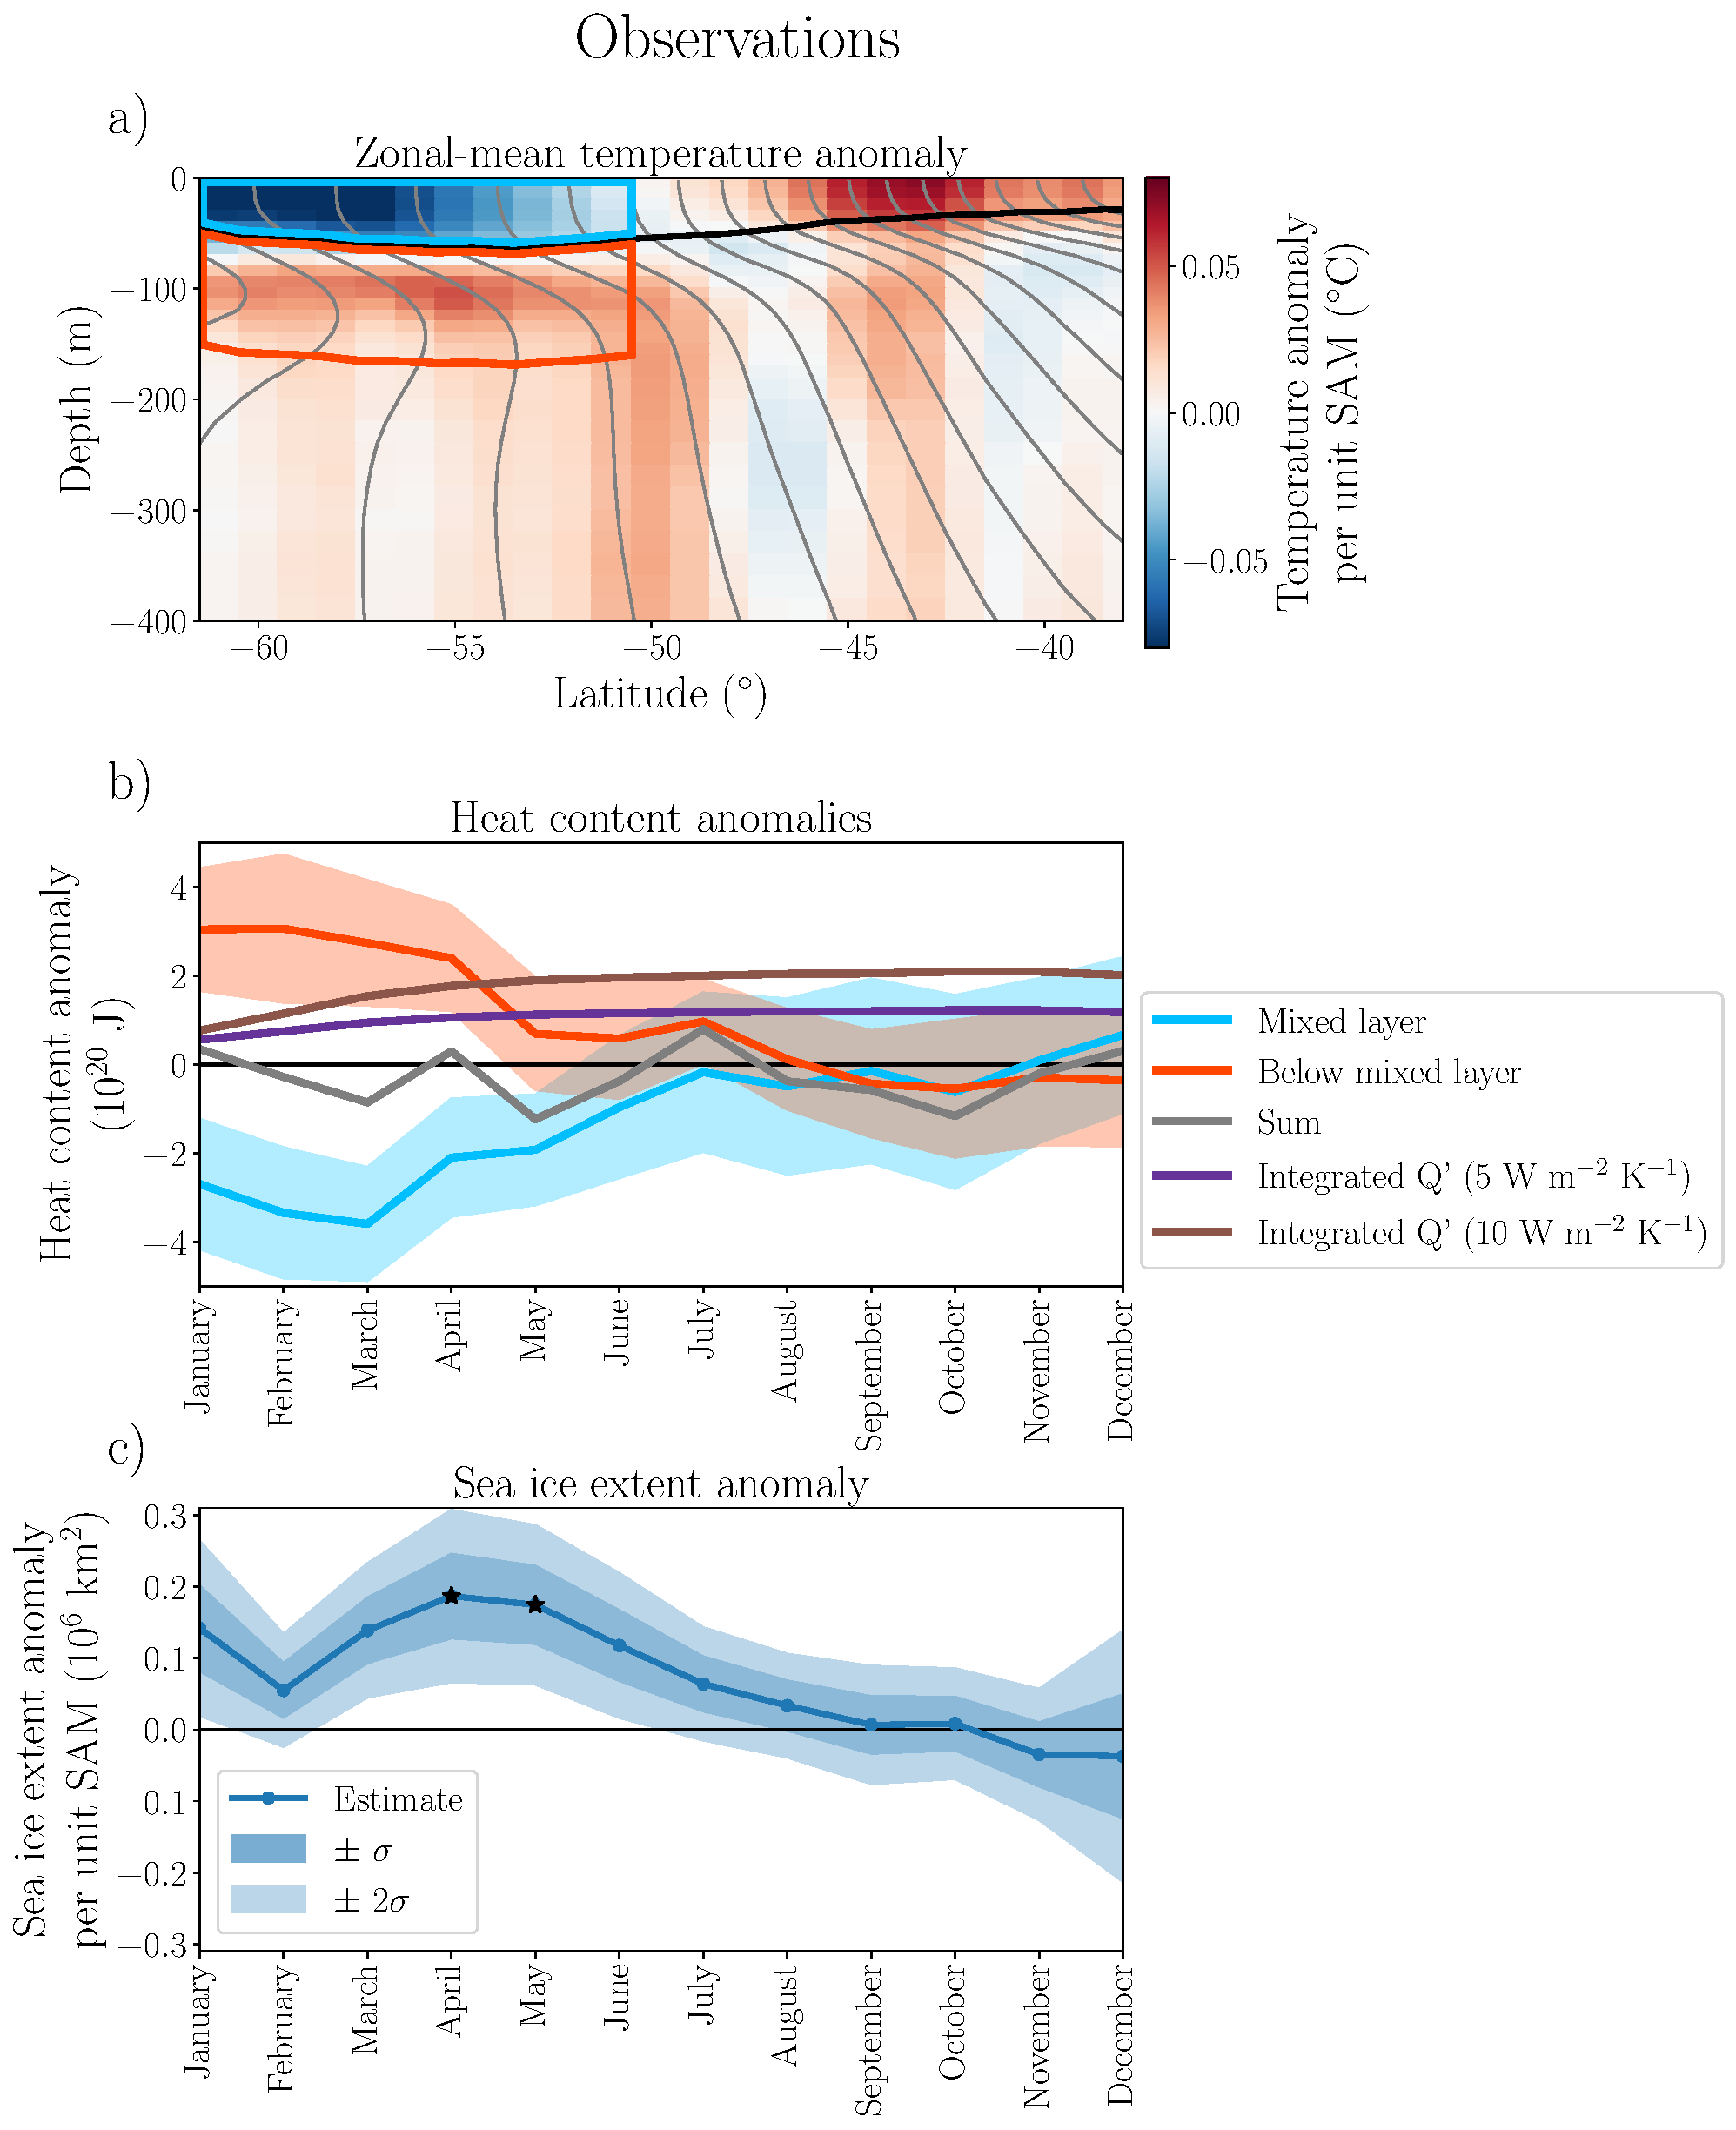
\includegraphics[width=0.9\textwidth]{figures/argo_regression_OHC_anomalies_and_time_series.pdf}
        \caption{a) Zonal-mean temperature anomaly in February per unit DJF SAM from an Argo-derived dataset. Also plotted is the climatological zonal-mean ocean temperature in February with a contour interval of 1$^{\circ}$C (grey contours), the climatological zonal-mean mixed layer depth in February (solid black line) and September (dashed black line) from \citet{Holte2017}. Blue and red boxes represent the regions in which the mixed layer and below mixed layer heat content anomalies are calculated in February.
        b) Heat content anomalies per unit SAM for cooling in the mixed layer (blue) and warming below (red). The colors are matched to the boxes shown in a. Integrated anomalous surface heat flux estimates for surface heat flux values of 5 and 10 W m$^{-2}$ K$^{-1}$ are shown by the purple and brown lines respectively.
        c) Sea ice extent anomaly per unit DJF SAM calculated using detrended time-series. Shaded regions show $\pm$ error estimate for the regression coefficient. Using the unmodified time-series does not qualitatively change the result.}
        \label{fig:argo_regression_OHC_anomalies_and_time_series}
    \end{center}
\end{figure}



The analysis presented by \citet{Doddridge2017} (their figure 3c) showed a transient increase in sea ice extent due to the summertime SAM. As in \citet{Doddridge2017}, we use the Sea Ice Index, version 2 produced by \citet{Fetterer2016} to assess sea ice extent and the National Oceanic and Atmospheric Administration (NOAA) Optimal Interpolation, version 2 dataset for sea ice concentration and SST \citep{Reynolds2002}. Repeating the analysis from \citet{Doddridge2017} with the additional data now available does not qualitatively alter the conclusions; the sea ice extent anomaly is largest in April, and then decreases, becoming negative by the end of the year (see figure \ref{fig:argo_regression_OHC_anomalies_and_time_series}c). However, due to the substantial interannual variability, the negative anomaly is not statistically discernible from zero. We are therefore unable to find evidence supporting the influence of our mechanism on wintertime sea ice extent in the observational record.

While our observational analysis is consistent with enhanced vertical mixing driving these zonal-mean temperature anomalies, it is not conclusive. In order to further explore the driving mechanism behind the observed vertical dipole in anomalous zonal-mean temperature, we turn to numerical models.


% section analysis_of_observations (end)


\section{Analysis of an idealized channel model of the ACC and its seasonal ice zone} % (fold)
\label{sec:analysis_of_an_idealised_channel_model}

We now turn to an idealized channel model of the ACC and its seasonal ice zone to further explore the response of the Southern Ocean to summertime perturbations in the westerly winds. Using a model allows us to diagnose heat budgets and isolate mechanisms driving change.  A snapshot of the model state in October (austral spring) is shown in figure \ref{fig:T_snapshot_3D}, which clearly highlights the eddying nature of the flow field.

The model is a reentrant channel, 3,200 km wide, 1,200 km long, and 4 km deep. The bathymetry for this model consists of a 300 m deep continental shelf at the southern boundary, which then slopes down to a flat bottom at 4,000 m depth for the rest of the domain. The horizontal resolution is 4 km and so resolves the oceanic mesoscale eddy field, which has been shown to play a leading-order role in the dynamics of the Southern Ocean \citep[see e.g.][]{Marshall2003,Marshall2012b,Munday2013}. Further details of our numerical setup can be found in \citet{Doddridge2019a}. While our model includes an interactive sea ice \citep{Losch2010} it lacks an interactive atmosphere, which precludes the study of coupled ocean-atmosphere phenomena. We use a repeating seasonal cycle of surface forcings that are derived from the Co-ordinated Ocean-Ice Reference Experiments (CORE) Corrected Normal Year Forcing Version 2.0 (CNYF) \citep{Large2004}.

The MITgcm \citep{Marshall1997,Marshall1997b} is used to solve the equations of motion, and the scientific Python stack to analyze the output \citep{Hoyer2017,Hunter2007,Kluyver2016,Perez2007,VanDerWalt2011}.


\begin{figure}[!ht]
    \begin{center}
        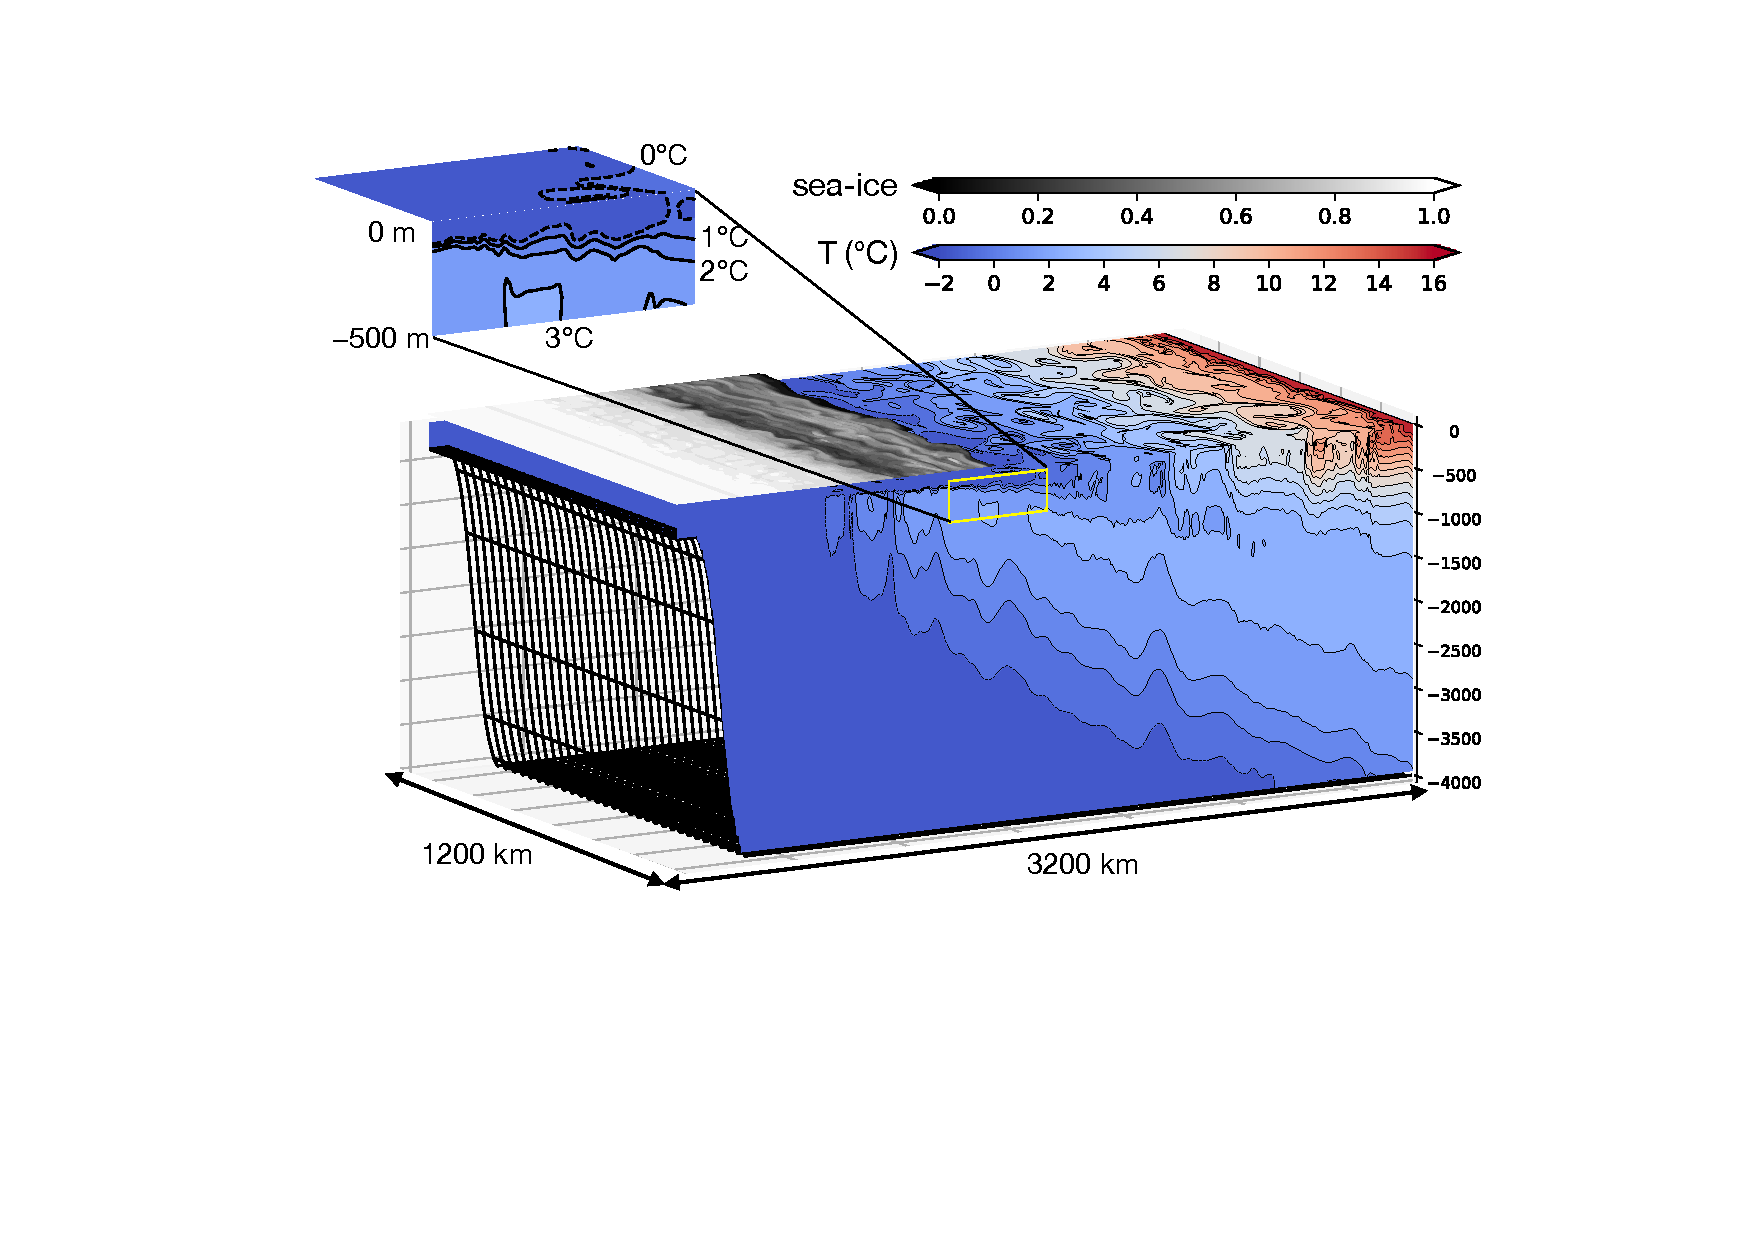
\includegraphics[width=0.9\textwidth]{figures/T_snapshot_3D.pdf}
        \caption{Snapshot of the temperature and sea ice fields in October (austral spring) from our idealized reentrant eddy-resolving channel model using MITgcm \citep{Marshall1997,Marshall1997b}. The model is driven by Coordinated Ocean Research Experiments Corrected Normal Year Forcing winds and fluxes. Note the presence of cold, fresh water at the surface in the region of the seasonal ice zone and a pronounced temperature inversion below.}
        \label{fig:T_snapshot_3D}
    \end{center}
\end{figure}


We begin by analyzing ensembles of idealized channel model simulations. After spinning up to a statistical equilibrium, we create two ensembles, one to establish the control and the other the perturbation about the control. To create a member of the perturbation ensemble we restart the model from a checkpoint with altered summertime zonal winds, surface air temperature, and surface humidity that mimic the positive phase of the SAM (see \citet{Doddridge2019a} for details of the perturbations). In our idealized model we represent only the strengthening of the zonal winds, neglecting the potential impact of a meridional shift \citep[c.f.][]{Waugh2019}. This means that we do not expect the channel model to reproduce the patch of surface warming seen in the observations (figure \ref{fig:argo_regression_OHC_anomalies_and_time_series}).


We use six snapshots from the control simulation as initial conditions for the perturbation ensemble members, with each set of initial conditions separated from the previous state by one year of model time. The control ensemble is created by using the same checkpoints, but continuing the simulation without altering the atmospheric fields. Averaging multiple ensemble members helps to reduce the impact of the vigorous mesoscale eddy field on our results.


One month after applying the wind perturbation the mixed layer is deeper and colder in the perturbation ensemble than the control ensemble (figures \ref{fig:channel_model_mld_anoms} and \ref{fig:channel_model_zonal_mean_one_month_with_heat_budget}a) \citep[c.f.][]{Sallee2010}. The mixed layer depth in our idealized channel model is calculated calculated using the density-based criterion of \citet{Kara2000} with $\Delta$T = 0.8$^{\circ}$C. There is also a region of anomalous warmth just below the zonal-mean mixed layer depth (figure \ref{fig:channel_model_zonal_mean_one_month_with_heat_budget}a). A heat budget shows that the negative temperature anomaly in the mixed layer and the positive temperature anomaly in the region below are both predominantly caused by enhanced vertical diffusion (figure \ref{fig:channel_model_zonal_mean_one_month_with_heat_budget}b). Both horizontal and vertical advection contribute to the cooling in the mixed layer, suggesting that the advective mechanisms proposed by \citet{Ferreira2015} and \citet{Purich2016} are also active in this model. However, the advective contributions are approximately an order of magnitude smaller than the cooling due to vertical diffusion (figure \ref{fig:channel_model_zonal_mean_one_month_with_heat_budget}b). The dominance of vertical mixing is further corroborated by the integrated ocean heat content anomalies (figure \ref{fig:channel_model_OHC_and_ice_anoms}). During the first summer the anomalous cooling in the mixed layer is slightly larger than the magnitude of the anomalous warming below the zonal-mean mixed layer depth, consistent with a small contribution from advection.


\begin{figure}[!ht]
	\begin{center}
		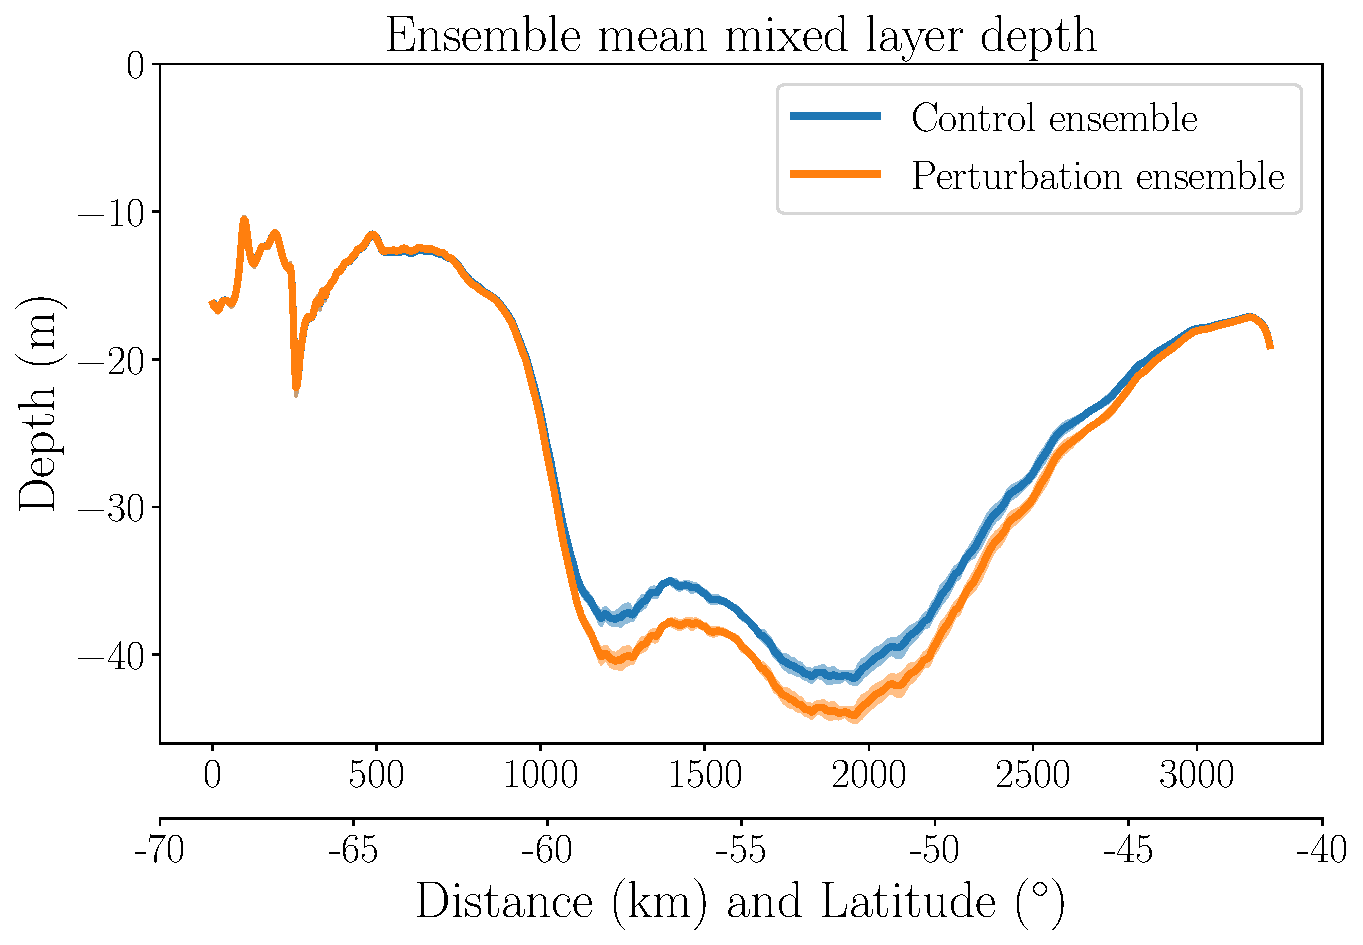
\includegraphics[width=0.7\textwidth]{figures/channel_model_mld_anoms.pdf}
		\caption{Zonal-mean, ensemble-mean mixed layer depth from our idealized channel model, one month after applying the surface forcing perturbations. The mixed layer is deeper in the perturbation ensemble due to enhanced near surface mixing caused by the strengthened zonal wind. Shading indicates the standard error of the mean, calculated as the standard deviation of the ensemble divided by the square root of six, the number of ensemble members.}
		\label{fig:channel_model_mld_anoms}
	\end{center}
\end{figure}


As predicted, there is an anomalous flux of heat into the ocean through the surface (not shown), which causes the total upper ocean heat content anomaly to increase (green line, figure \ref{fig:channel_model_OHC_and_ice_anoms}). During autumn, the mixed layer deepens and returns the anomalously warm water below the zonal-mean mixed layer depth to the surface. In conjunction with the anomalous surface heat fluxes, this causes the mixed layer to become anomalously warm during the winter months (blue line, figure \ref{fig:channel_model_OHC_and_ice_anoms}) and reduces sea ice volume (red line, figure \ref{fig:channel_model_OHC_and_ice_anoms}). Our idealized channel model fails to reproduce the transient increase in sea ice extent found by \citet{Doddridge2017} in the observations. This is likely due to the sea ice edge being too far south to be substantially affected by the anomalously cold SST; by the time the sea ice edge extends far enough north to interact with the SST anomaly, the mixed layer has become anomalously warm.






\begin{figure}[!ht]
    \begin{center}
        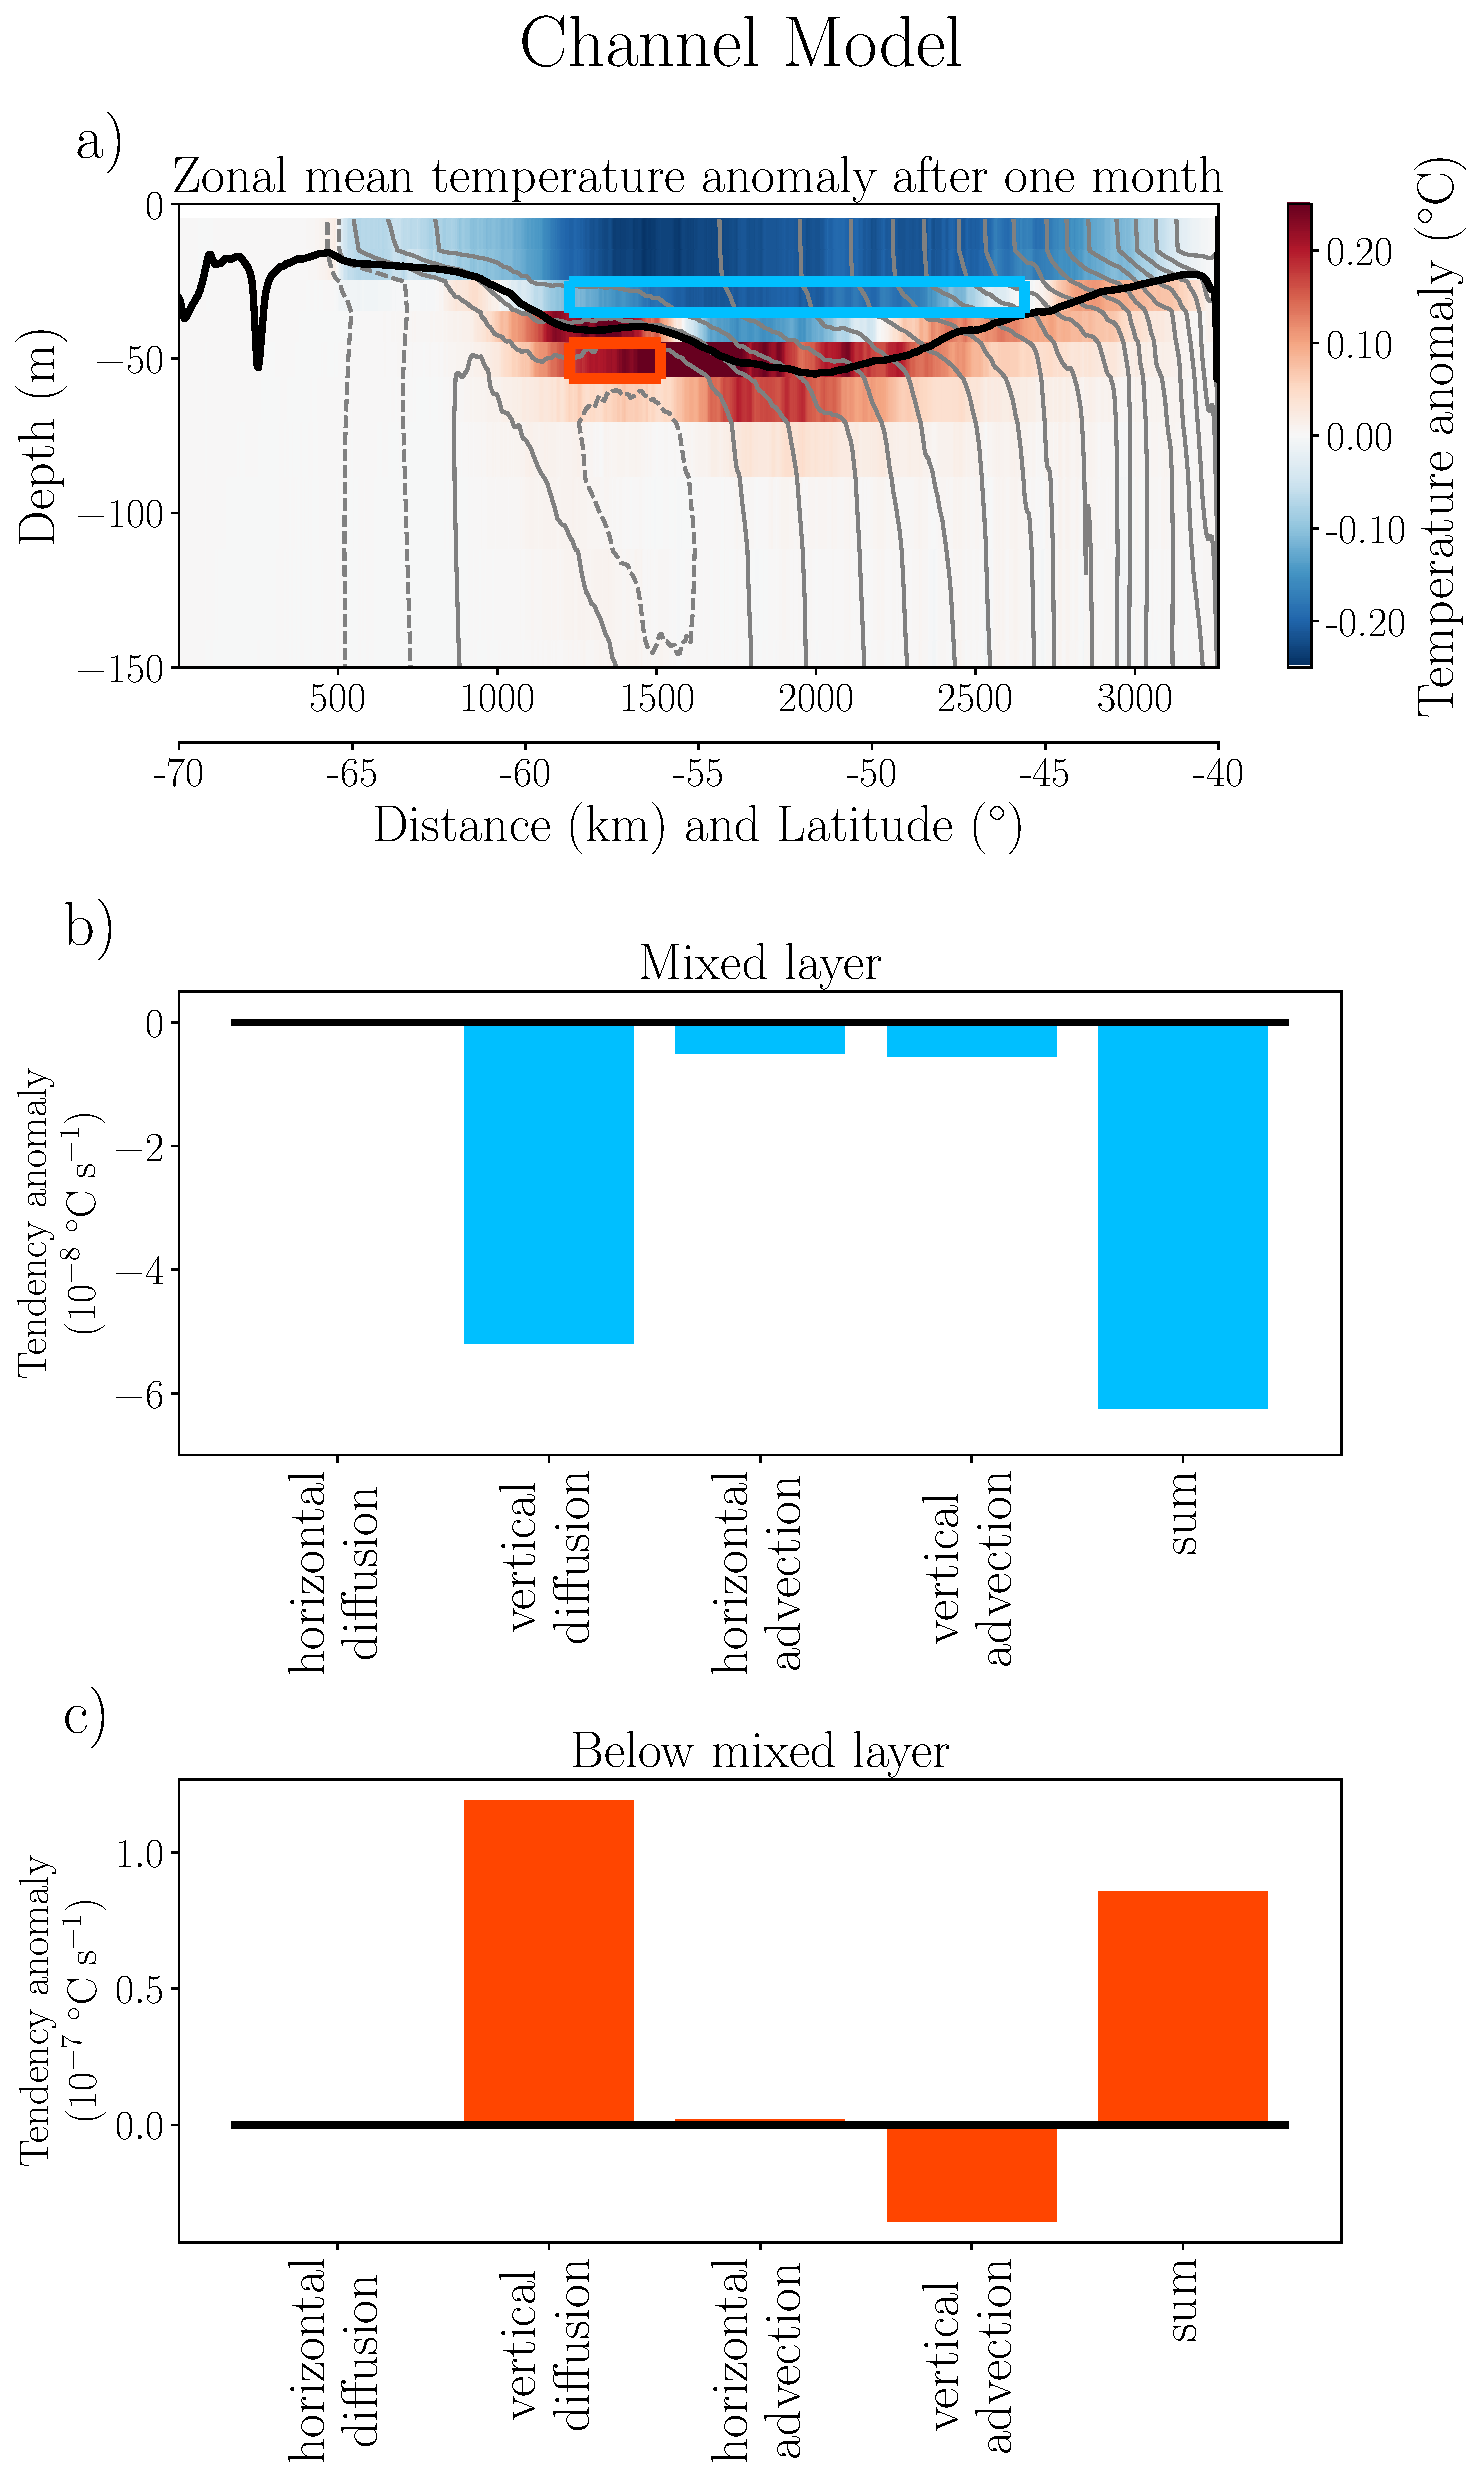
\includegraphics[width=0.7\textwidth]{figures/channel_model_zonal_mean_one_month_with_heat_budget.pdf}
        \caption{Results from the eddying channel model one month after the wind perturbation is applied. a) Zonal-mean temperature anomalies after one month (colors). The thin gray contours shows the climatological zonal-mean temperature field from the control ensemble in February at $\pm0.5$, $\pm1.5 \dots$ $^{\circ}$C, with negative contours dashed. The thick black line shows the zonal-mean mixed layer depth from the perturbation ensemble. b) Zonal-mean heat budget for the region of the mixed layer outlined by the blue box in a) showing that vertical diffusion dominates the cooling tendency. c) Zonal-mean heat budget for the region below the zonal-mean mixed layer depth outlined by the red box in a) showing that vertical diffusion dominates the warming. The vertical advection contribution is consistent with the enhanced upwelling predicted by \citet{Purich2016}.}
        \label{fig:channel_model_zonal_mean_one_month_with_heat_budget}
    \end{center}
\end{figure}

\begin{figure}[!ht]
    \begin{center}
        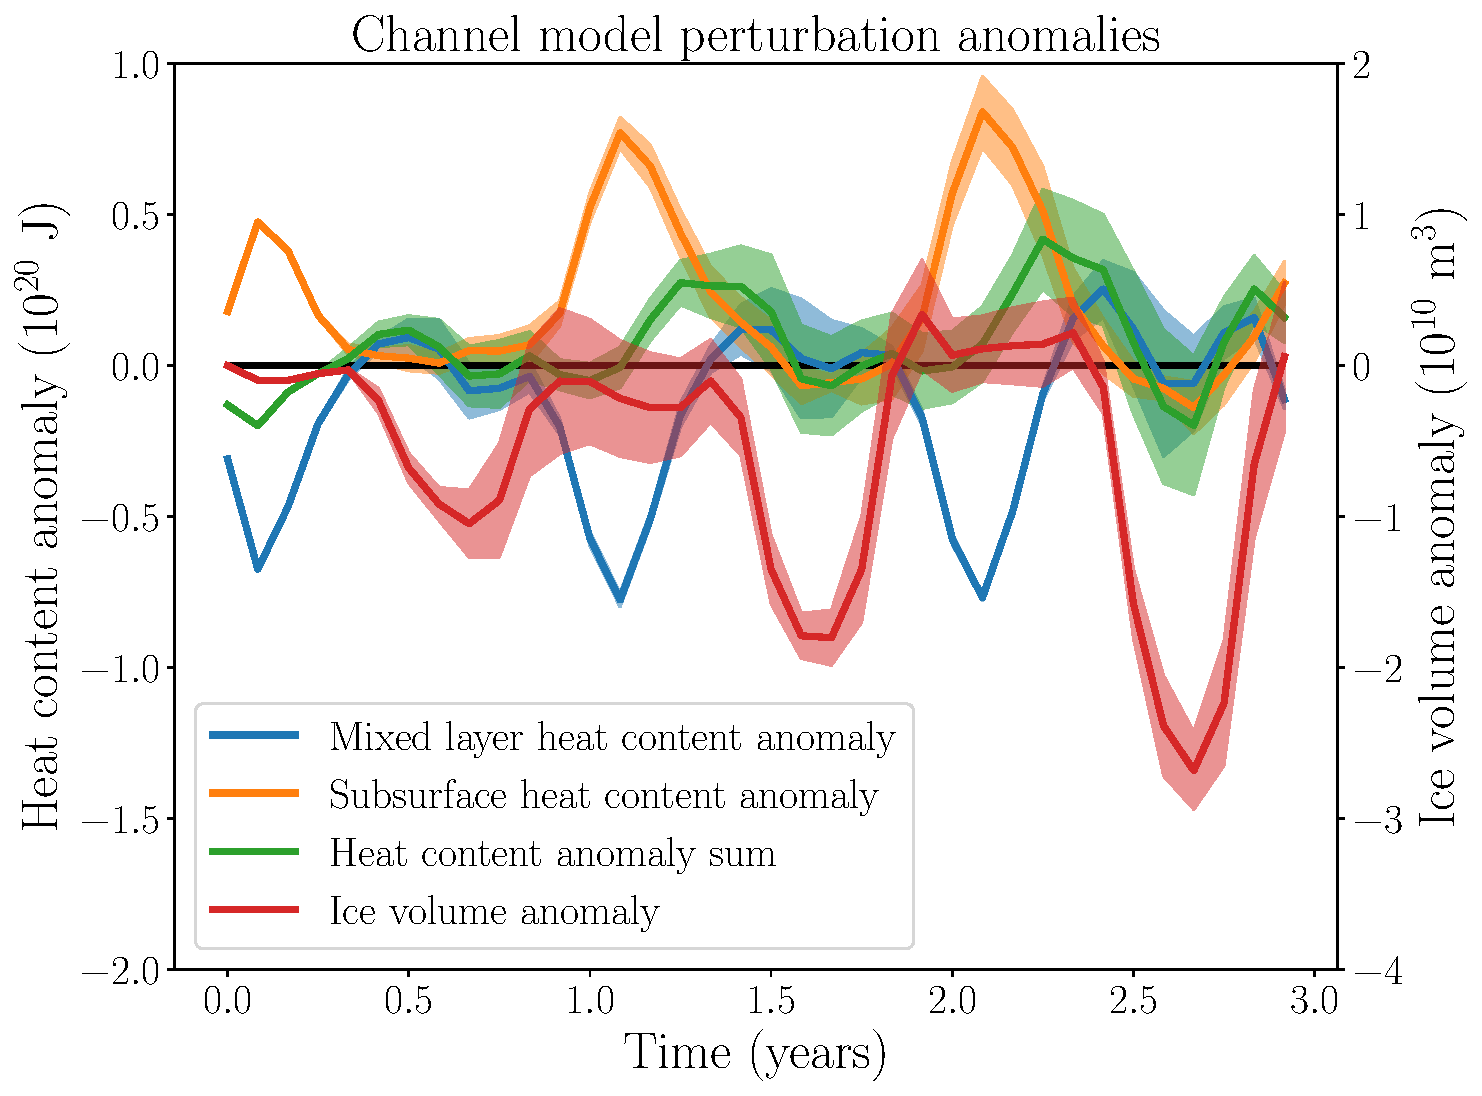
\includegraphics[width=0.7\textwidth]{figures/channel_model_OHC_and_ice_anoms.pdf}
        \caption{Mixed layer heat content anomaly for the channel model (blue line), for the 100 m thick region below the mixed layer (orange line), the sum of these two (green line), and sea ice volume anomaly (red line, right hand axis). Shading represents one standard deviation of the ensemble. The x-axis is time (years) and the y-axis is either Joules or cubic meters.}
        \label{fig:channel_model_OHC_and_ice_anoms}
    \end{center}
\end{figure}

% section analysis_of_an_idealised_channel_model (end)


\section{Analysis of the GISS coupled climate model} % (fold)
\label{sec:analysis_of_a_global_coupled_model}

While the zonal-mean temperature anomalies in our idealized channel model have much in common with those found in the observations, both in pattern and amplitude, the idealized nature of that model raises questions about how widely applicable the results are. We therefore seek to test our proposed mechanism in another model, one that is global and fully coupled, with interactive atmosphere, ice, and ocean components. We use the most recent National Aeronautics and Space Administration (NASA) Goddard Institute for Space Studies (GISS) global coupled model, Model E2.1, in the configuration described by \citet{Doddridge2019a}. A major caveat is that due to the added complexity, this model is run at a much coarser resolution and mesoscale eddies are parameterized rather than explicitly resolved. The model includes a Gent-McWilliams style eddy parameterization \citep{Gent1990,Gent1995} with a flow-dependent variable eddy diffusivity. Further details of the model and our numerical setup can be found in \citet{Doddridge2019a}, \citet{Kelley2020}, and \citet{Miller2020}.

The climatology of the control configuration of this model closely resembles the observed climatology of the Southern Ocean; figure \ref{fig:GISS_overview} shows the surface climatology in the Southern Ocean for the summertime sea ice minimum in February (a) and the wintertime sea ice maximum in September (b). From an equilibrated preindustrial control simulation we spawn an ensemble of perturbation experiments by imposing a stratospheric ozone hole mimicking the conditions in the 1990s (see \citet{Doddridge2019a} for details of the ozone hole perturbation). The imposed ozone depletion causes the summertime SAM to become anomalously positive and enhances the summertime westerly winds \citep{Polvani2011}. Once again we construct a control ensemble by combining the equivalent unperturbed simulations and define the anomaly as the difference between the two ensemble means. We will now use these ensembles to assess the influence of our mechanism in a global coupled model.






\begin{figure}[!ht]
    \begin{center}
        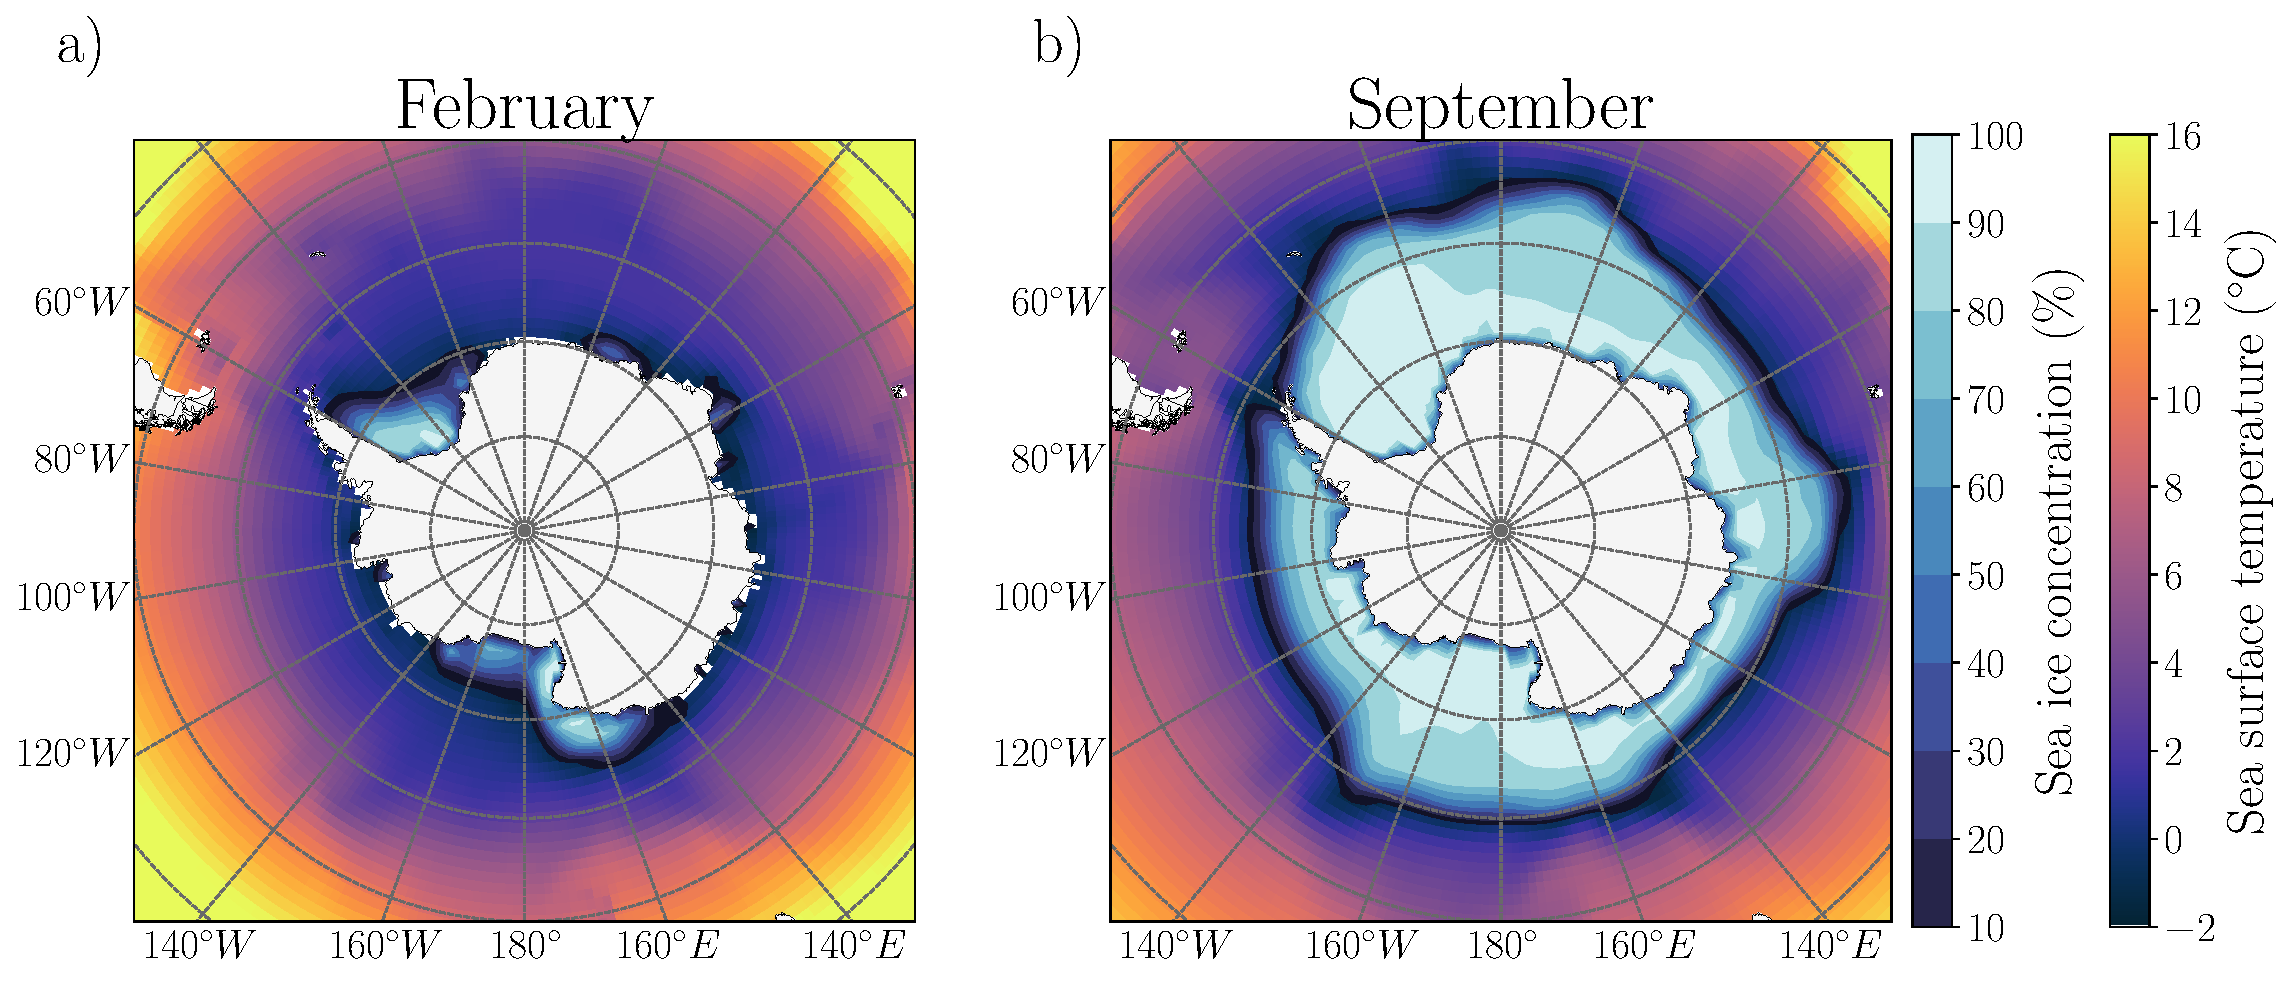
\includegraphics[width=0.99\textwidth]{figures/GISS_overview.pdf}
        \caption{Southern Ocean climatology from the preindustrial control run of the GISS global coupled model. a) shows SST and sea ice concentration in February, the summertime sea ice minimum. b) shows SST and sea ice concentration in September, the wintertime sea ice maximum.}
        \label{fig:GISS_overview}
    \end{center}
\end{figure}


The zonal-mean temperature perturbation clearly shows a vertical dipole (figure \ref{fig:GISS_zm_temperature_anoms_heat_budget}a). A heat budget for the mixed layer reveals that the cooling is largely driven by advection, with diffusion making a small contribution (figure \ref{fig:GISS_zm_temperature_anoms_heat_budget}b). The warming is located below the zonal-mean mixed layer depth from the control ensemble, and our heat budget analysis reveals that diffusion is the largest contributor to this warming (figure \ref{fig:GISS_zm_temperature_anoms_heat_budget}c). Calculating the ocean heat content anomaly in the mixed layer and the region below the mixed layer shows that the cooling in the mixed layer is larger than the warming below, consistent with advectively driven cooling. Because the model fields required to decompose the advective contribution into horizontal and vertical components are not available, we cannot assess which of the two advective hypotheses this model supports.


% Although advection dominates the cooling signal in the mixed layer, our global coupled model still shows mixing induced warming below the zonal-mean mixed layer depth, consistent with our proposed mechanism.




\begin{figure}[!ht]
    \begin{center}
        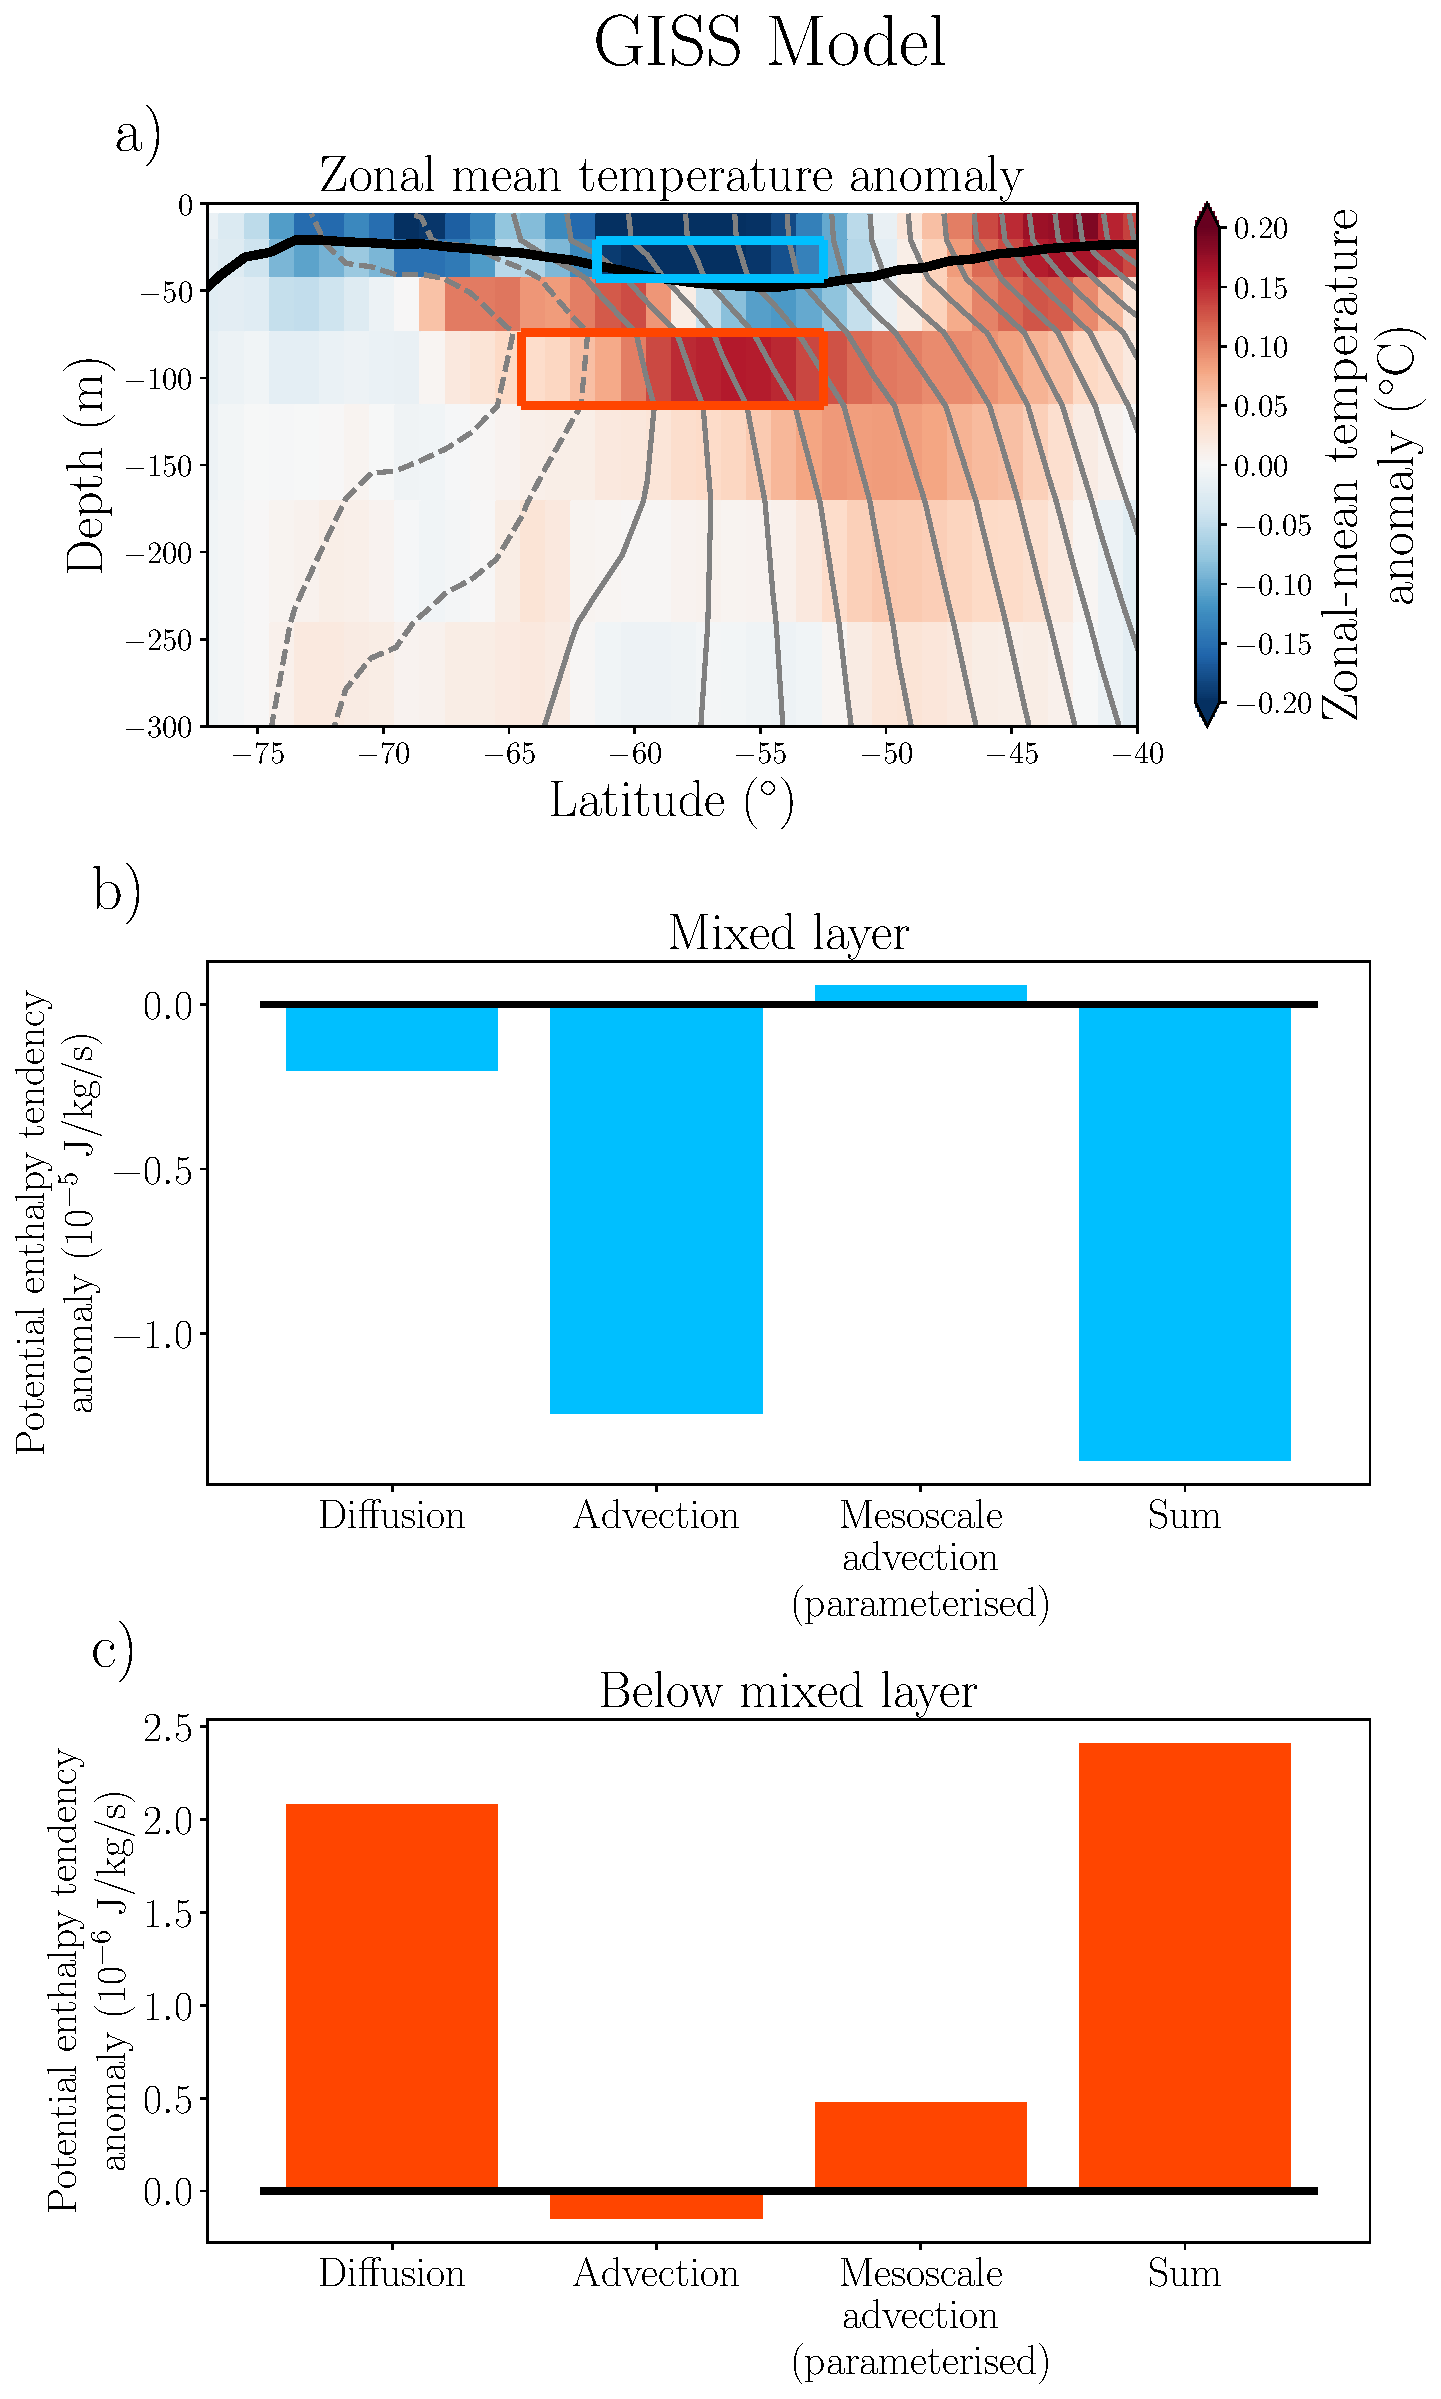
\includegraphics[width=0.7\textwidth]{figures/GISS_zm_temperature_anoms_heat_budget.pdf}
        \caption{a) Zonal-mean temperature anomaly in the GISS model in February of the second year of the simulation. The gray contours show the climatological February temperature field from the control ensemble with contours at 0, $\pm$1, $\pm2$, ... $^{\circ}$C, negative and zero contours are dashed. The thick black line represents the zonal-mean mixed layer depth from the perturbation ensemble.
        b) Zonal-mean anomalous heat budget for a region in the mixed layer in February of the second year, shown by the blue rectangle in a). Advection makes the largest contribution to the anomalous cooling. Mixing contributes only about one fifth as much cooling as advection.
        c) Zonal-mean anomalous heat budget for a region below the zonal-mean mixed layer depth in February of the second year. The region is shown by the red rectangle in a). Mixing is largely responsible for the anomalous warming. (Note that the vertical scale in c is an order of magnitude smaller than b.)}
        \label{fig:GISS_zm_temperature_anoms_heat_budget}
    \end{center}
\end{figure}


% MAYBE INCLUDE THE FIRST THREE YEARS OF ML OHC AND BML OHC ANOMALIES? SHOWS CLEARLY THAT ONE GOES UP, THE OTHER GOES DOWN? XXX



To allow for easier comparison with the observational analysis in section \ref{sec:analysis_of_observations} and \citet{Doddridge2017}, we will switch from analyzing differences between the control and perturbation ensembles to performing regression analyses on the control ensemble. We begin by defining an analogous SAM index to the observational index from \citet{Marshall2003a}. We then compute lagged linear correlations between this SAM index and the zonal-mean temperature field. The predicted zonal-mean temperature anomaly from a +1 SAM is shown in figure \ref{fig:GISS_regression_OHC_anomalies_and_time_series}a. The ocean heat content anomalies implied by these temperature changes are plotted in figure \ref{fig:GISS_regression_OHC_anomalies_and_time_series}b, and show that the cooling in the mixed layer is substantially larger than the warming below. The difference between the two heat content anomalies is consistent with the heat budget analysis that showed advection played a substantial role in cooling the mixed layer (figure \ref{fig:GISS_zm_temperature_anoms_heat_budget}b). To assess the sea ice response to SAM perturbations we regress sea ice area and sea ice volume against the summertime SAM index. We find a transient increase in both area and volume that peaks in May, following which the area anomaly decreases to zero and the volume anomaly becomes negative (figure \ref{fig:GISS_regression_OHC_anomalies_and_time_series}c). Our analysis suggests that positive perturbations to the summertime SAM may reduce sea ice volume at the wintertime peak in sea ice. However, the lack of statistical significance means that we are unable to draw robust conclusions about the change in sea ice volume from these simulations.


% If we assume a surface heat flux feedback of 5-10 Wm$^{-2}$ consistent with recent observational estimates \citep{Hausmann2016}, then we can calculate the expected anomalous heat flux. The integrated expected anomalous heat flux over the twelve months from January to December is approximately equal to the change in upper ocean heat content (figure \ref{fig:GISS_regression_OHC_anomalies_and_time_series}b).


\begin{figure}[!ht]
    \begin{center}
        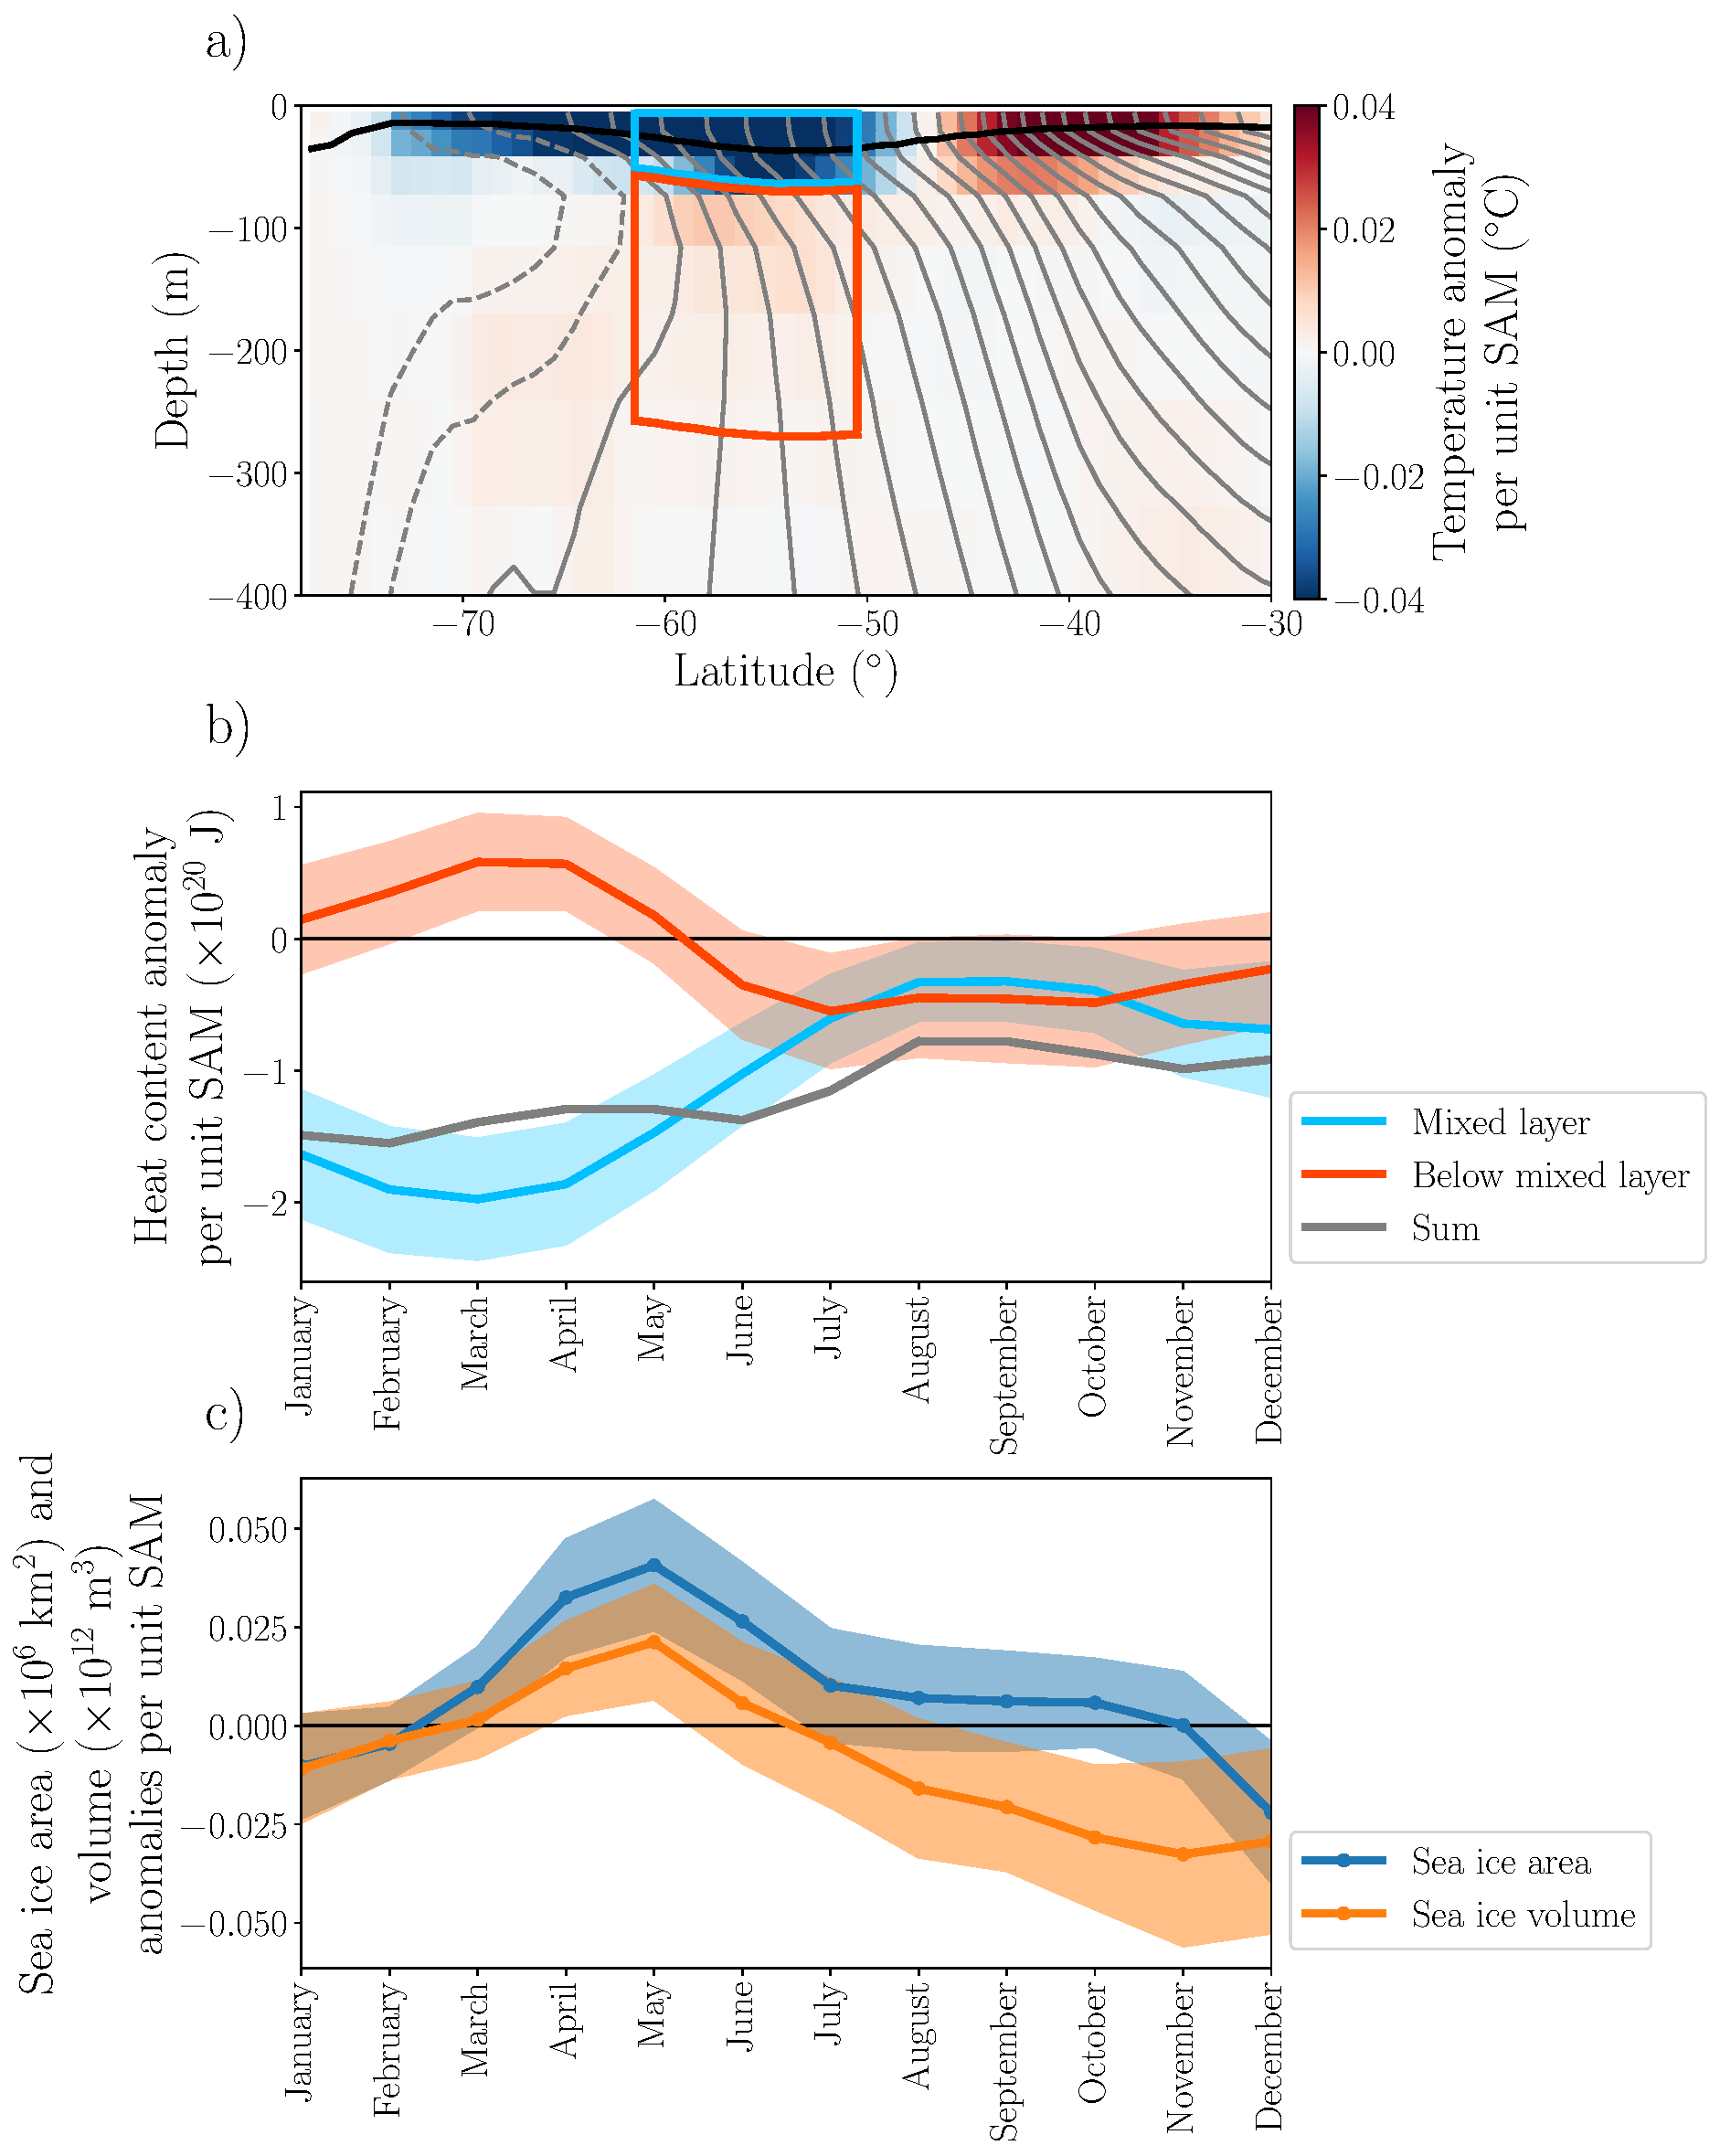
\includegraphics[width=0.9\textwidth]{figures/GISS_regression_OHC_anomalies_and_time_series.pdf}
        \caption{Correlations between SAM and other model fields from the GISS control simulation. a) Zonal-mean February temperature anomaly per unit DJF SAM. Gray contours show climatological zonal-mean temperature field in February with contours at 0, $\pm$1, $\pm2$, ... $^{\circ}$C, negative and zero contours are dashed. Black line represents climatological zonal-mean mixed layer depth in February from the control ensemble. b) Ocean heat content anomalies calculated using the zonal-mean temperature perturbations and regions shown in a). Blue line represents mixed layer box, red line represents box below mixed layer. Consistent with the diagnostics in figure \ref{fig:GISS_zm_temperature_anoms_heat_budget}, the sum of the two heat content anomalies is negative (gray line), showing that vertical redistribution is not the only process cooling the mixed layer. c) The sea ice area (blue) and volume (orange) anomalies per unit SAM. Both show a transient increase, but only sea ice volume shows a reduction in the following winter. After applying a Bonferroni correction none of the regression coefficients are statistically discernible from zero.}
        \label{fig:GISS_regression_OHC_anomalies_and_time_series}
    \end{center}
\end{figure}







% section analysis_of_a_global_coupled_model (end)



% \section{Case study} % (fold)
% \label{sec:case_study}
% Try and find a particular year and region that shows this mechanism clearly. 

% The Wedell Sea in 2012 is a candidate.

% % section case_study (end)




\section{Discussion and Conclusions} % (fold)
\label{sec:discussion}

We have proposed a new mechanism through which summertime wind perturbations can affect ocean temperature and sea ice over a seasonal timescale. According to our mechanism, strengthened summertime winds lead to anomalous vertical mixing, which cools the mixed layer and warms the ocean just beneath mixed layer. Due to the anomalously cold sea surface, anomalous air-sea heat fluxes transfer additional heat into the surface ocean. As the mixed layer deepens during the autumn months, the combined effect of the anomalous air-sea heat fluxes and entrainment of anomalously warm subsurface water causes the mixed layer to become anomalously warm. This would likely lead to a reduction in sea ice during the winter months, either in ice volume or ice extent, or both.


It has previously been proposed that the surface cooling in response to strengthened westerly winds is primarily due to horizontal advection \citep{Ferreira2015} or vertical advection \citep{Purich2016}. Our analysis of the observations suggests that enhanced vertical diffusion plays the leading role in creating both the cold SST anomaly and the warm subsurface temperature anomaly. However, due to inadequacies in data we are unable to rule out an advective contribution to the observed surface cooling signal. Our idealized channel model does not support an advective mechanism; the heat budget (figure \ref{fig:channel_model_zonal_mean_one_month_with_heat_budget}b) clearly shows that anomalous vertical mixing is the dominant cause of the cold SST anomaly, with only minor contributions from both horizontal and vertical advection. This enhanced vertical mixing is also responsible for subsurface warming. In our global coupled model, the subsurface warming is similarly due to enhanced vertical mixing, but the mixed layer cooling is mostly due to advection, with only a small contribution from mixing. The relative importance of our proposed mixing-based mechanism and the previously proposed advective mechanisms \citep{Ferreira2015,Purich2016} is therefore model dependent. Given the observational uncertainty and model dependence, it is difficult to conclusively state which mechanism is most important in the Southern Ocean. That said, we lend strong credence to the highly resolved channel calculations presented here -- because the relevant dynamics is resolved -- and believe that enhanced vertical diffusion is likely more important than either horizontal or vertical advection.

% Due to a lack of available model fields, we are unable to decompose the advective contribution into horizontal  and vertical components and can therefore not assess which of the proposed advective mechanisms dominates in our coupled model \citep{Ferreira2015,Purich2016}.


Our observational analysis and our coupled global model both show that the summertime SAM has  little impact on the wintertime sea ice extent. However, both our idealized channel model and our global coupled model show a reduction in sea ice volume in the winter following anomalously strong summertime westerlies. These results suggest that sea ice volume is more sensitive to summertime winds than sea ice extent. Unfortunately, we are unable to assess the relationship between summertime winds and sea ice volume in the observations due to the lack of a long-term time-series for sea ice volume in the Southern Ocean. If, as our modeling results suggest, stronger summertime westerlies do cause a reduction in sea ice volume in the following winter, then a positive DJF SAM may precondition sea ice for a rapid retreat in the following spring. Indeed there was a remarkable reduction in sea ice extent observed in the austral spring of 2016 (September-October-November) \citep{Jones2016,Parkinson2012,Scambos2018} which followed an unusually large and positive SAM in the summer of 2015 which may have preconditioned Antarctic sea ice for the rapid springtime retreat the following year. That said, the 2016 decline has been linked to numerous factors including anomalous meridional winds and heat advection in the atmosphere \citep{Schlosser2017}, El Ni\~no \citep{Stuecker2017}, and to the Southern Annular Mode (SAM) \citep{Doddridge2017}. The breadth of proposed explanations is testament to the complexity of the southern cryosphere. Exploring the contribution of our mechanism to sea ice changes in specific years or locations presents an exciting avenue for future work.

Our focus on summertime winds is motivated by the observed changes in the summertime SAM \citep{Marshall2003a}, and the potential for seasonal reemergence of the sequestered heat. During winter the mixed layer is substantially deeper \citep{Holte2017}, and the stratification is such that additional mixing at the base of the mixed layer would warm the surface waters. It is only during the summer, when a shallow thermally stratified layer forms a cap above the previous winter's mixed layer, that additional mixing can cool the surface. We have therefore focused on the impacts of enhanced zonal winds in the summertime.

Through our proposed mechanism, enhanced summertime winds drive anomalous near-surface diapycnal mixing. According to \citet{Sloyan2010}, summertime diapycnal mixing near the Subantarctic Front preconditions the ocean for the rapid development of deep mixed layers and efficient formation of Subantarctic Mode Water (SAMW) and Antarctic Intermediate Water (AAIW). Our mechanism may therefore increase the volume of SAMW and AAIW formed \citep[c.f.][]{Gao2018}. Further analysis of the role of summertime wind anomalies on the formation of SAMW and AAIW are beyond the scope of this contribution.

In conclusion, we have presented a novel mechanism that predicts a non-monotonic SST response to summertime wind perturbations: initially the sea surface cools before warming in the winter months as heat that was sequestered below the surface is returned to the surface mixed layer. Our mechanism predicts that enhanced summertime westerlies will increase sea ice cover during the autumn and reduce sea ice volume during winter; predictions that are supported by our modeling studies and observational analysis.

%% In all cases, if there is only one entry of this type within
%% the higher level heading, use the star form: 
%%
% \section{Section title}
% \subsection*{subsection}
% text...
% \section{Section title}

%vs

% \section{Section title}
% \subsection{subsection one}
% text...
% \subsection{subsection two}
% \section{Section title}

%%%
% \section{First primary heading}

% \subsection{First secondary heading}

% \subsubsection{First tertiary heading}

% \paragraph{First quaternary heading}

%%%%%%%%%%%%%%%%%%%%%%%%%%%%%%%%%%%%%%%%%%%%%%%%%%%%%%%%%%%%%%%%%%%%%
% DATA AVAILABILITY STATEMENT
%%%%%%%%%%%%%%%%%%%%%%%%%%%%%%%%%%%%%%%%%%%%%%%%%%%%%%%%%%%%%%%%%%%%%
% The data availability statement is where authors should describe how the data underlying the findings within the article can be accessed and reused. 
% Authors should attempt to provide unrestricted access to all data and materials underlying reported findings. If data access is restricted, 
% authors must mention this in the statement.
%
\datastatement
All observational datasets used can be obtained by following the directions in the cited articles. Model configurations are described in detail in the text and cited articles. Due to the expense of publicly hosting large datasets, the model output is not publicly available. Interested readers should contact the corresponding author for further information or access.

%%%%%%%%%%%%%%%%%%%%%%%%%%%%%%%%%%%%%%%%%%%%%%%%%%%%%%%%%%%%%%%%%%%%%
% ACKNOWLEDGMENTS
%%%%%%%%%%%%%%%%%%%%%%%%%%%%%%%%%%%%%%%%%%%%%%%%%%%%%%%%%%%%%%%%%%%%%
%
\acknowledgments
We thank Alex Haumann for helpful comments on an earlier draft. E. Doddridge acknowledges support from the NSF's Antarctic program. J. Marshall acknowledges support from the MIT-GISS collaborative agreement and the NSF Polar Antarctic Program. H. Song is supported by Yonsei University Research Fund (2018-22-0053) and National Research Foundation of Korea (NRF) grant funded by Korea government (MSIST) (NRF-2019R1C1C1003663).


%%%%%%%%%%%%%%%%%%%%%%%%%%%%%%%%%%%%%%%%%%%%%%%%%%%%%%%%%%%%%%%%%%%%%
% APPENDIXES
%%%%%%%%%%%%%%%%%%%%%%%%%%%%%%%%%%%%%%%%%%%%%%%%%%%%%%%%%%%%%%%%%%%%%
%
% Use \appendix if there is only one appendix.
%\appendix

% Use \appendix[A], \appendix[B], if you have multiple appendixes.
%\appendix[A]

%% Appendix title is necessary! For appendix title:
%\appendixtitle{}

%%% Appendix section numbering (note, skip \section and begin with \subsection)
% \subsection{First primary heading}

% \subsubsection{First secondary heading}

% \paragraph{First tertiary heading}

%% Important!
%\appendcaption{<appendix letter and number>}{<caption>} 
%must be used for figures and tables in appendixes, e.g.,
%
%\begin{figure}
%\noindent\includegraphics[width=19pc,angle=0]{figure01.pdf}\\
%\appendcaption{A1}{Caption here.}
%\end{figure}
%
% All appendix figures/tables should be placed in order AFTER the main figures/tables, i.e., tables, appendix tables, figures, appendix figures.
%
%%%%%%%%%%%%%%%%%%%%%%%%%%%%%%%%%%%%%%%%%%%%%%%%%%%%%%%%%%%%%%%%%%%%%
% REFERENCES
%%%%%%%%%%%%%%%%%%%%%%%%%%%%%%%%%%%%%%%%%%%%%%%%%%%%%%%%%%%%%%%%%%%%%
% Make your BibTeX bibliography by using these commands:
\bibliographystyle{ametsoc2014}
\bibliography{library}


%%%%%%%%%%%%%%%%%%%%%%%%%%%%%%%%%%%%%%%%%%%%%%%%%%%%%%%%%%%%%%%%%%%%%
% TABLES
%%%%%%%%%%%%%%%%%%%%%%%%%%%%%%%%%%%%%%%%%%%%%%%%%%%%%%%%%%%%%%%%%%%%%
%% Enter tables at the end of the document, before figures.
%%
%
%\begin{table}[t]
%\caption{This is a sample table caption and table layout.  Enter as many tables as
%  necessary at the end of your manuscript. Table from Lorenz (1963).}\label{t1}
%\begin{center}
%\begin{tabular}{ccccrrcrc}
%\hline\hline
%$N$ & $X$ & $Y$ & $Z$\\
%\hline
% 0000 & 0000 & 0010 & 0000 \\
% 0005 & 0004 & 0012 & 0000 \\
% 0010 & 0009 & 0020 & 0000 \\
% 0015 & 0016 & 0036 & 0002 \\
% 0020 & 0030 & 0066 & 0007 \\
% 0025 & 0054 & 0115 & 0024 \\
%\hline
%\end{tabular}
%\end{center}
%\end{table}

%%%%%%%%%%%%%%%%%%%%%%%%%%%%%%%%%%%%%%%%%%%%%%%%%%%%%%%%%%%%%%%%%%%%%
% FIGURES
%%%%%%%%%%%%%%%%%%%%%%%%%%%%%%%%%%%%%%%%%%%%%%%%%%%%%%%%%%%%%%%%%%%%%
%% Enter figures at the end of the document, after tables.
%%
%
%\begin{figure}[t]
%  \noindent\includegraphics[width=19pc,angle=0]{figure01.pdf}\\
%  \caption{Enter the caption for your figure here.  Repeat as
%  necessary for each of your figures. Figure from \protect\cite{Knutti2008}.}\label{f1}
%\end{figure}

\end{document}